\documentclass[12pt,a4paper]{report}

\usepackage[utf8]{inputenc}
\usepackage[T1]{fontenc}

\usepackage{amsmath,amssymb,amsthm}
\usepackage{mathtools}
\usepackage{geometry}
\usepackage{graphicx}
\usepackage{xcolor}
\usepackage{booktabs}
\usepackage{array}
\usepackage{longtable}
\usepackage{multirow}
\usepackage{pgfplots}
\usepackage{tikz}
\usepackage{pgfplotstable}
\usetikzlibrary{arrows.meta,decorations.pathreplacing,patterns,calc,shapes,positioning,fit,backgrounds}
\pgfplotsset{compat=1.18}
\usepackage{fancyhdr}
\usepackage{titlesec}
\usepackage{tcolorbox}
\tcbuselibrary{theorems,skins,breakable,most}
\usepackage{enumitem}
\usepackage{hyperref}
\usepackage{cleveref}
\usepackage{caption}
\usepackage{subcaption}
\usepackage{float}
\usepackage{setspace}
\usepackage{parskip}
\usepackage{mathrsfs}
\usepackage{bm}
\usepackage{cancel}

\geometry{
  top=2.5cm, bottom=2.5cm,
  left=3cm, right=2.5cm,
  headheight=15pt
}

\definecolor{azuloscuro}{RGB}{0,51,102}
\definecolor{azulmedio}{RGB}{0,102,179}
\definecolor{azulclaro}{RGB}{173,216,230}
\definecolor{rojoalerta}{RGB}{180,0,0}
\definecolor{verdematematica}{RGB}{0,100,0}
\definecolor{amarillonota}{RGB}{255,248,220}
\definecolor{grisclaro}{RGB}{245,245,245}
\definecolor{naranjaejemplo}{RGB}{200,80,0}
\definecolor{moradoteorema}{RGB}{80,0,120}

\hypersetup{
  colorlinks=true,
  linkcolor=azuloscuro,
  citecolor=verdematematica,
  urlcolor=azulmedio,
  pdftitle={Capítulo 11 -- Heteroscedasticidad: Gujarati},
  pdfauthor={Econometría Avanzada},
  pdfsubject={Econometría}
}

\tcbset{
  defstyle/.style={
    enhanced,breakable,
    colback=grisclaro,colframe=azuloscuro,
    fonttitle=\bfseries\color{white},
    attach boxed title to top left={yshift=-2mm,xshift=4mm},
    boxed title style={colback=azuloscuro,sharp corners},
    sharp corners,
    left=6pt,right=6pt,top=6pt,bottom=6pt
  },
  teoremastyle/.style={
    enhanced,breakable,
    colback=moradoteorema!5,colframe=moradoteorema,
    fonttitle=\bfseries\color{white},
    attach boxed title to top left={yshift=-2mm,xshift=4mm},
    boxed title style={colback=moradoteorema,sharp corners},
    sharp corners
  },
  ejemplostyle/.style={
    enhanced,breakable,
    colback=naranjaejemplo!6,colframe=naranjaejemplo,
    fonttitle=\bfseries\color{white},
    attach boxed title to top left={yshift=-2mm,xshift=4mm},
    boxed title style={colback=naranjaejemplo,sharp corners},
    sharp corners
  },
  alertastyle/.style={
    enhanced,breakable,
    colback=rojoalerta!6,colframe=rojoalerta,
    fonttitle=\bfseries\color{white},
    attach boxed title to top left={yshift=-2mm,xshift=4mm},
    boxed title style={colback=rojoalerta,sharp corners},
    sharp corners
  },
  notastyle/.style={
    enhanced,breakable,
    colback=amarillonota,colframe=azulmedio!70,
    fonttitle=\bfseries\color{azuloscuro},
    attach boxed title to top left={yshift=-2mm,xshift=4mm},
    boxed title style={colback=azulmedio!70,sharp corners},
    sharp corners
  },
  ejerciciostyle/.style={
    enhanced,breakable,
    colback=verdematematica!5,colframe=verdematematica,
    fonttitle=\bfseries\color{white},
    attach boxed title to top left={yshift=-2mm,xshift=4mm},
    boxed title style={colback=verdematematica,sharp corners},
    sharp corners
  }
}

\newtheorem{teorema}{Teorema}[section]
\newtheorem{proposicion}[teorema]{Proposición}
\newtheorem{corolario}[teorema]{Corolario}
\newtheorem{lema}[teorema]{Lema}
\theoremstyle{definition}
\newtheorem{definicion}{Definición}[section]
\newtheorem{ejemplo}{Ejemplo}[section]
\newtheorem{ejercicio}{Ejercicio}[section]
\theoremstyle{remark}
\newtheorem{observacion}{Observación}[section]

\pagestyle{fancy}
\fancyhf{}
\fancyhead[L]{\small\textcolor{azuloscuro}{\textbf{Econometría -- Gujarati}}}
\fancyhead[R]{\small\textcolor{azuloscuro}{Capítulo 11: Heteroscedasticidad}}
\fancyfoot[C]{\thepage}
\renewcommand{\headrulewidth}{0.6pt}
\renewcommand{\headrule}{\hbox to\headwidth{\color{azuloscuro}\leaders\hrule height \headrulewidth\hfill}}

\titleformat{\chapter}[display]
  {\normalfont\huge\bfseries\color{azuloscuro}}
  {\chaptertitlename\ \thechapter}{20pt}{\Huge}
\titleformat{\section}
  {\normalfont\Large\bfseries\color{azuloscuro}}
  {\thesection}{1em}{}[\titlerule]
\titleformat{\subsection}
  {\normalfont\large\bfseries\color{azulmedio}}
  {\thesubsection}{1em}{}
\titleformat{\subsubsection}
  {\normalfont\normalsize\bfseries\color{naranjaejemplo}}
  {\thesubsubsection}{1em}{}

\newcommand{\E}{\mathbb{E}}
\newcommand{\Var}{\mathrm{Var}}
\newcommand{\Cov}{\mathrm{Cov}}
\newcommand{\betahat}{\hat{\beta}}
\newcommand{\uhat}{\hat{u}}
\newcommand{\sigmahat}{\hat{\sigma}}
\newcommand{\yhat}{\hat{Y}}
\newcommand{\BLUE}{\text{BLUE}}
\newcommand{\OLS}{\text{MCO}}
\newcommand{\GLS}{\text{MCG}}
\newcommand{\WLS}{\text{MCP}}
\newcommand{\iid}{\overset{iid}{\sim}}
\newcommand{\plim}{\operatorname{plim}}

\onehalfspacing

\begin{document}

\begin{titlepage}
  \begin{tikzpicture}[remember picture, overlay]
    \fill[azuloscuro] (current page.north west) rectangle ([yshift=-6cm]current page.north east);
    \fill[azulmedio] ([yshift=-6cm]current page.north west) rectangle ([yshift=-6.5cm]current page.north east);
    \fill[azulclaro!50] ([yshift=-6.5cm]current page.north west) rectangle ([yshift=-7cm]current page.north east);
    \node[anchor=north, text=white, font=\Huge\bfseries, align=center]
      at ([yshift=-1.5cm]current page.north) {ECONOMETRÍA};
    \node[anchor=north, text=white!85, font=\large, align=center]
      at ([yshift=-3cm]current page.north) {Damodar N. Gujarati -- Análisis Riguroso y Completo};
    \node[anchor=north, text=white, font=\huge\bfseries, align=center]
      at ([yshift=-4.8cm]current page.north) {CAPÍTULO 11};
  \end{tikzpicture}

  \vspace{7.5cm}

  \begin{center}
    {\fontsize{26}{32}\selectfont\bfseries\color{azuloscuro}
    Heteroscedasticidad}\\[0.5cm]
    {\Large\color{azulmedio}
    ¿Qué ocurre cuando la varianza del error no es constante?}\\[1.5cm]

    \begin{tcolorbox}[width=0.85\textwidth,colback=grisclaro,colframe=azuloscuro,sharp corners]
      \centering
      \textbf{Contenido del documento}\\[0.3cm]
      \small
      \begin{tabular}{ll}
        \S 11.1 & Naturaleza de la heteroscedasticidad \\
        \S 11.2 & Estimación por MCO bajo heteroscedasticidad \\
        \S 11.3 & Mínimos Cuadrados Generalizados (MCG) \\
        \S 11.4 & Consecuencias formales del uso de MCO \\
        \S 11.5 & Detección de la heteroscedasticidad \\
        \S 11.6 & Medidas remediales \\
        \S 11.7 & Ejemplos finales con datos reales \\
        \S 11.8 & Ejercicios resueltos \\
        \S\S A   & Anexo de fórmulas derivadas paso a paso \\
      \end{tabular}
    \end{tcolorbox}

    \vfill
    {\color{azuloscuro}\rule{0.6\textwidth}{1.2pt}}\\[0.4cm]
    {\large\textbf{Documento Académico de Referencia}}\\
    {\normalsize Teoría $\cdot$ Demostraciones $\cdot$ Ejemplos Numéricos $\cdot$ Ejercicios Resueltos}
  \end{center}
\end{titlepage}

\tableofcontents
\clearpage

\chapter{Heteroscedasticidad: Fundamentos, Detección y Corrección}

\section{Naturaleza de la Heteroscedasticidad}

\subsection{El Modelo Lineal Clásico y el Supuesto de Homocedasticidad}

El Modelo Lineal Clásico (MLC) de regresión múltiple puede escribirse matricialmente como:
\begin{equation}
  \mathbf{y} = \mathbf{X}\boldsymbol{\beta} + \mathbf{u}
  \label{eq:mlc}
\end{equation}
donde $\mathbf{y}$ es el vector $(n \times 1)$ de la variable dependiente, $\mathbf{X}$ es la matriz $(n \times k)$ de regresores (incluyendo la constante), $\boldsymbol{\beta}$ es el vector $(k \times 1)$ de parámetros desconocidos, y $\mathbf{u}$ es el vector $(n \times 1)$ de perturbaciones estocásticas.

Entre los supuestos estándar, el de \textbf{homocedasticidad} establece que:
\begin{equation}
  \E(u_i^2) = \sigma^2 \quad \forall\, i = 1, 2, \ldots, n
  \label{eq:homo}
\end{equation}

O de forma matricial, la estructura de varianza-covarianza de las perturbaciones es:
\begin{equation}
  \E(\mathbf{u}\mathbf{u}') = \sigma^2 \mathbf{I}_n
  \label{eq:homo_matricial}
\end{equation}

\begin{tcolorbox}[defstyle, title={Definición 11.1: Homocedasticidad}]
  Se dice que un modelo presenta \textbf{homocedasticidad} cuando la varianza de las perturbaciones es constante e igual a $\sigma^2$ para todas las observaciones, independientemente de los valores que tomen las variables explicativas. Formalmente: $\Var(u_i \mid X_i) = \sigma^2$ para todo $i$.
\end{tcolorbox}

\begin{tcolorbox}[defstyle, title={Definición 11.2: Heteroscedasticidad}]
  Se dice que un modelo presenta \textbf{heteroscedasticidad} cuando la varianza de las perturbaciones no es constante, sino que varía a lo largo de las observaciones:
  \begin{equation}
    \E(u_i^2) = \sigma_i^2, \quad \sigma_i^2 \neq \sigma_j^2 \text{ para al menos algún } i \neq j
    \label{eq:hetero}
  \end{equation}
  La estructura de varianza-covarianza pasa a ser una matriz diagonal no escalar:
  \begin{equation}
    \E(\mathbf{u}\mathbf{u}') = \boldsymbol{\Omega} =
    \begin{pmatrix}
      \sigma_1^2 & 0 & \cdots & 0 \\
      0 & \sigma_2^2 & \cdots & 0 \\
      \vdots & \vdots & \ddots & \vdots \\
      0 & 0 & \cdots & \sigma_n^2
    \end{pmatrix}
    \label{eq:omega}
  \end{equation}
\end{tcolorbox}

\subsection{Representación Gráfica Comparativa}

\begin{figure}[H]
  \centering
  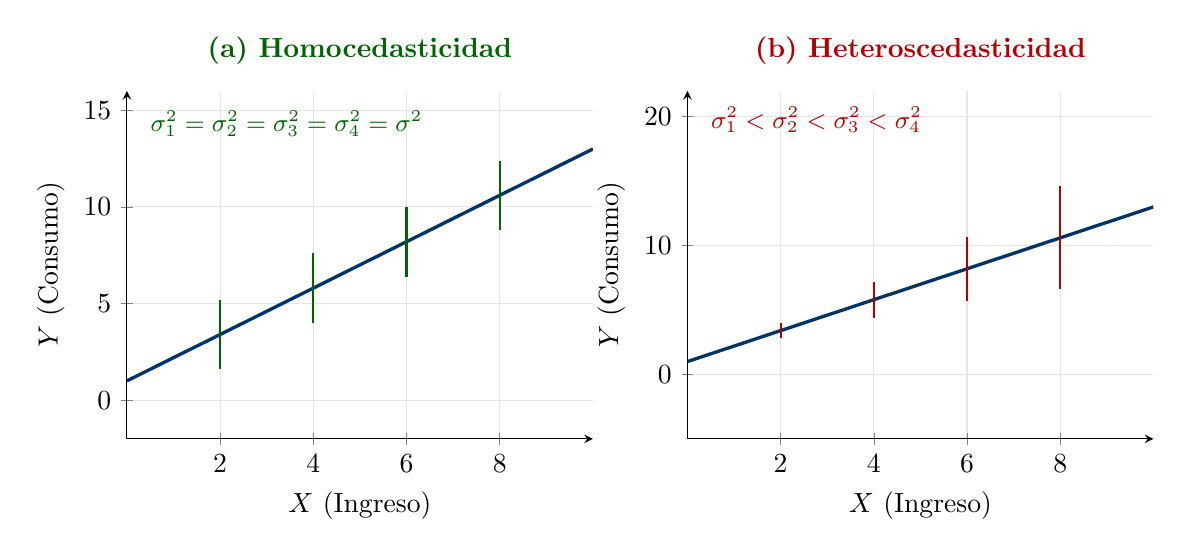
\begin{tikzpicture}
    \begin{axis}[
      name=ax1,
      width=7.5cm, height=6cm,
      xlabel={$X$ (Ingreso)},
      ylabel={$Y$ (Consumo)},
      title={\textbf{(a) Homocedasticidad}},
      title style={color=verdematematica},
      xmin=0, xmax=10, ymin=-2, ymax=16,
      xtick={2,4,6,8},
      axis lines=left,
      grid=both, grid style={gray!20},
    ]
      \addplot[azuloscuro, very thick, domain=0:10] {1.2*x + 1};
      \foreach \x/\base in {2/3.4, 4/5.8, 6/8.2, 8/10.6} {
        \addplot[verdematematica!60, fill=verdematematica!15, opacity=0.5]
          coordinates {(\x,\base-1.8)(\x,\base+1.8)};
        \addplot[verdematematica, thick] coordinates {(\x,\base-1.8)(\x,\base+1.8)};
      }
      \node[anchor=north west, font=\small, color=verdematematica] at (axis cs:0.3,15.5)
        {$\sigma_1^2 = \sigma_2^2 = \sigma_3^2 = \sigma_4^2 = \sigma^2$};
    \end{axis}

    \begin{axis}[
      name=ax2,
      at={(ax1.east)}, anchor=west, xshift=1.2cm,
      width=7.5cm, height=6cm,
      xlabel={$X$ (Ingreso)},
      ylabel={$Y$ (Consumo)},
      title={\textbf{(b) Heteroscedasticidad}},
      title style={color=rojoalerta},
      xmin=0, xmax=10, ymin=-5, ymax=22,
      xtick={2,4,6,8},
      axis lines=left,
      grid=both, grid style={gray!20},
    ]
      \addplot[azuloscuro, very thick, domain=0:10] {1.2*x + 1};
      \foreach \x/\base/\spread in {2/3.4/0.6, 4/5.8/1.4, 6/8.2/2.5, 8/10.6/4.0} {
        \addplot[rojoalerta!60, fill=rojoalerta!15, opacity=0.5]
          coordinates {(\x,\base-\spread)(\x,\base+\spread)};
        \addplot[rojoalerta, thick] coordinates {(\x,\base-\spread)(\x,\base+\spread)};
      }
      \node[anchor=north west, font=\small, color=rojoalerta] at (axis cs:0.3,21.5)
        {$\sigma_1^2 < \sigma_2^2 < \sigma_3^2 < \sigma_4^2$};
    \end{axis}
  \end{tikzpicture}
  \caption{Comparación gráfica entre homocedasticidad y heteroscedasticidad. Las barras verticales representan la dispersión condicional de $Y$ dado $X$. En el panel (a) la dispersión es constante; en el panel (b) crece con $X$, patrón típico en datos de ingreso-consumo.}
  \label{fig:homo_vs_hetero}
\end{figure}

\subsection{Causas Económicas de la Heteroscedasticidad}

\begin{tcolorbox}[notastyle, title={Causas Principales}]
  \begin{enumerate}[label=\textbf{\arabic*.}]
    \item \textbf{Discrecionalidad en el ingreso (Efecto escala):} Las familias con ingresos altos tienen mayor discrecionalidad en su gasto, exhibiendo mayor variabilidad en el consumo que las familias de bajos ingresos. Si $\sigma_i^2 = f(\text{Ingreso}_i)$, con $f' > 0$, la varianza crece con el nivel de ingresos.

    \item \textbf{Mejora en técnicas de recolección de datos:} A medida que el tiempo avanza y las metodologías estadísticas mejoran (censos, encuestas), los errores de medición se reducen, disminuyendo $\sigma_i^2$ a lo largo del tiempo.

    \item \textbf{Efecto aprendizaje:} En estudios de productividad o errores de predicción, la varianza tiende a decrecer conforme los agentes acumulan experiencia.

    \item \textbf{Valores atípicos (Outliers):} Una sola observación extrema puede sesgar drásticamente las estimaciones de la varianza, especialmente con muestras pequeñas.

    \item \textbf{Errores de especificación:} Si el modelo verdadero es $Y_i = \beta_1 + \beta_2 X_i^2 + u_i$ pero se estima $Y_i = \alpha_1 + \alpha_2 X_i + v_i$, el término $v_i$ absorberá el efecto cuadrático omitido, generando una varianza que aumenta con $X$.

    \item \textbf{Asimetría distribucional:} Variables como el ingreso, la riqueza, o el tamaño de las empresas tienen distribuciones muy asimétricas hacia la derecha. Las observaciones en la cola derecha son escasas pero de alta variabilidad, induciendo heteroscedasticidad.

    \item \textbf{Datos de corte transversal (Cross-section):} Cuando se mezclan unidades muy heterogéneas (ej. empresas con ventas de \$1M y otras con ventas de \$50,000M), la varianza naturalmente difiere entre grupos.
  \end{enumerate}
\end{tcolorbox}

\subsection{Formas Funcionales Comunes de Heteroscedasticidad}

En la práctica, se asume que $\sigma_i^2$ es una función de las variables explicativas. Las especificaciones más comunes son:

\begin{align}
  \sigma_i^2 &= \sigma^2 X_i^{\alpha} & &\text{(Park: potencia)} \label{eq:park_form}\\
  \sigma_i^2 &= \sigma^2 e^{\alpha X_i} & &\text{(exponencial)} \label{eq:exp_form}\\
  \sigma_i^2 &= (\alpha_0 + \alpha_1 X_i)^2 & &\text{(lineal en SD)} \label{eq:linear_sd}\\
  \sigma_i^2 &= \alpha_0 + \alpha_1 X_i^2 & &\text{(Glejser cuadrática)} \label{eq:glejser_form}
\end{align}

\begin{figure}[H]
  \centering
  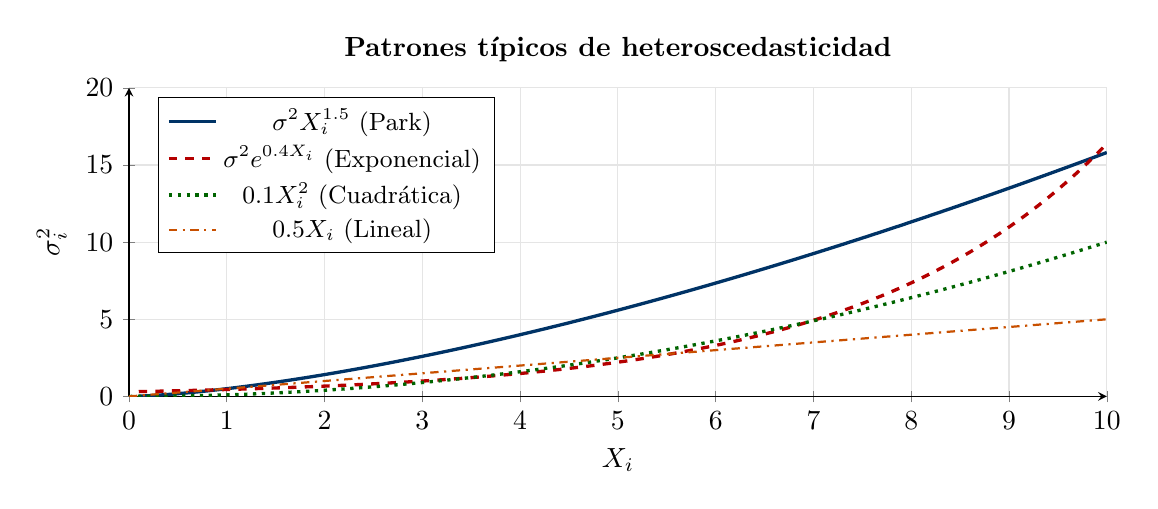
\begin{tikzpicture}
    \begin{axis}[
      width=14cm, height=5.5cm,
      xlabel={$X_i$},
      ylabel={$\sigma_i^2$},
      title={\textbf{Patrones típicos de heteroscedasticidad}},
      xmin=0, xmax=10, ymin=0, ymax=20,
      legend pos=north west,
      legend style={font=\small},
      grid=major, grid style={gray!20},
      axis lines=left,
    ]
      \addplot[azuloscuro, very thick, domain=0.1:10, samples=100] {0.5*x^1.5};
      \addlegendentry{$\sigma^2 X_i^{1.5}$ (Park)}
      \addplot[rojoalerta, very thick, dashed, domain=0.1:10, samples=100] {0.3*exp(0.4*x)};
      \addlegendentry{$\sigma^2 e^{0.4 X_i}$ (Exponencial)}
      \addplot[verdematematica, very thick, dotted, domain=0:10, samples=100] {0.1*x^2};
      \addlegendentry{$0.1 X_i^2$ (Cuadrática)}
      \addplot[naranjaejemplo, thick, dash dot, domain=0:10, samples=100] {0.5*x};
      \addlegendentry{$0.5 X_i$ (Lineal)}
    \end{axis}
  \end{tikzpicture}
  \caption{Distintas formas funcionales de la varianza heteroscedástica como función de la variable independiente $X_i$.}
  \label{fig:patrones_sigma}
\end{figure}

\section{Estimación por MCO en Presencia de Heteroscedasticidad}

\subsection{El Estimador MCO}

Para el modelo simple $Y_i = \beta_1 + \beta_2 X_i + u_i$, el estimador de mínimos cuadrados ordinarios minimiza la suma de cuadrados residuales sin ponderar:
\begin{equation}
  S(\beta_1, \beta_2) = \sum_{i=1}^n \uhat_i^2 = \sum_{i=1}^n (Y_i - \beta_1 - \beta_2 X_i)^2
  \label{eq:ols_obj}
\end{equation}

Derivando e igualando a cero (condiciones de primer orden):
\begin{align}
  \frac{\partial S}{\partial \beta_1} &= -2\sum_{i=1}^n (Y_i - \betahat_1 - \betahat_2 X_i) = 0 \label{eq:cpo1}\\
  \frac{\partial S}{\partial \beta_2} &= -2\sum_{i=1}^n X_i(Y_i - \betahat_1 - \betahat_2 X_i) = 0 \label{eq:cpo2}
\end{align}

Resolviendo el sistema de ecuaciones normales se obtiene:
\begin{equation}
  \betahat_2 = \frac{\sum_{i=1}^n x_i y_i}{\sum_{i=1}^n x_i^2} = \frac{\sum_{i=1}^n (X_i - \bar{X})(Y_i - \bar{Y})}{\sum_{i=1}^n (X_i - \bar{X})^2}
  \label{eq:beta2hat}
\end{equation}
donde $x_i = X_i - \bar{X}$ e $y_i = Y_i - \bar{Y}$ son las desviaciones respecto a la media.

\subsection{Propiedades del Estimador MCO bajo Heteroscedasticidad}

\begin{tcolorbox}[teoremastyle, title={Teorema 11.1: Insesgadez de MCO bajo Heteroscedasticidad}]
  \textbf{Enunciado:} Bajo heteroscedasticidad (pero manteniendo el supuesto de exogeneidad estricta $\E(\mathbf{u} \mid \mathbf{X}) = \mathbf{0}$), el estimador MCO sigue siendo insesgado:
  \begin{equation}
    \E(\betahat_{\OLS}) = \boldsymbol{\beta}
    \label{eq:insesgadez}
  \end{equation}

  \textbf{Demostración:}
  \begin{align*}
    \betahat_{\OLS} &= (\mathbf{X}'\mathbf{X})^{-1}\mathbf{X}'\mathbf{y}
    = (\mathbf{X}'\mathbf{X})^{-1}\mathbf{X}'(\mathbf{X}\boldsymbol{\beta} + \mathbf{u})\\
    &= \boldsymbol{\beta} + (\mathbf{X}'\mathbf{X})^{-1}\mathbf{X}'\mathbf{u}
  \end{align*}
  Tomando esperanza condicional en $\mathbf{X}$:
  \begin{align*}
    \E(\betahat_{\OLS} \mid \mathbf{X}) &= \boldsymbol{\beta} + (\mathbf{X}'\mathbf{X})^{-1}\mathbf{X}'\underbrace{\E(\mathbf{u} \mid \mathbf{X})}_{=\mathbf{0}} = \boldsymbol{\beta} \qquad \blacksquare
  \end{align*}
  La insesgadez \textbf{no depende} del supuesto de homocedasticidad, sino únicamente de la exogeneidad.
\end{tcolorbox}

\begin{tcolorbox}[alertastyle, title={Resultado Crítico: Fórmula de Varianza Incorrecta}]
  Bajo heteroscedasticidad, la verdadera matriz de varianza-covarianza del estimador MCO es:
  \begin{equation}
    \Var(\betahat_{\OLS} \mid \mathbf{X}) = (\mathbf{X}'\mathbf{X})^{-1}\mathbf{X}'\boldsymbol{\Omega}\mathbf{X}(\mathbf{X}'\mathbf{X})^{-1}
    \label{eq:sandwich}
  \end{equation}
  Esta es la célebre \textbf{fórmula sándwich} (sandwich formula). El software estadístico estándar, en cambio, calcula \textbf{erróneamente}:
  \begin{equation}
    \widehat{\Var}_{\text{conv}}(\betahat_{\OLS}) = \sigmahat^2 (\mathbf{X}'\mathbf{X})^{-1}
    \label{eq:var_conv}
  \end{equation}
  La diferencia entre \eqref{eq:sandwich} y \eqref{eq:var_conv} \textbf{invalida completamente} la inferencia estadística: pruebas $t$, pruebas $F$, intervalos de confianza.
\end{tcolorbox}

Para el caso bivariado, la varianza verdadera de $\betahat_2$ es:
\begin{equation}
  \Var(\betahat_2) = \frac{\sum_{i=1}^n x_i^2 \sigma_i^2}{\left(\sum_{i=1}^n x_i^2\right)^2}
  \label{eq:var_beta2_true}
\end{equation}
mientras que la fórmula convencional (incorrecta) asume:
\begin{equation}
  \widehat{\Var}_{\text{conv}}(\betahat_2) = \frac{\sigma^2}{\sum_{i=1}^n x_i^2}
  \label{eq:var_beta2_conv}
\end{equation}

\begin{tcolorbox}[teoremastyle, title={Teorema 11.2: Ineficiencia de MCO -- Gauss-Markov Modificado}]
  \textbf{Enunciado:} Bajo heteroscedasticidad, MCO \textbf{ya no es BLUE}. El estimador MCG (definido en la sección siguiente) tiene menor varianza que MCO para todo $\boldsymbol{\beta}$.

  \textbf{Interpretación económica:} MCO asigna pesos iguales $w_i = 1/n$ a todas las observaciones. Esto es subóptimo: las observaciones con varianza pequeña ($\sigma_i^2$ pequeño) contienen información más precisa sobre la línea de regresión verdadera. Ignorar esta diferencia de calidad informativa produce estimadores menos precisos.
\end{tcolorbox}

\begin{figure}[H]
  \centering
  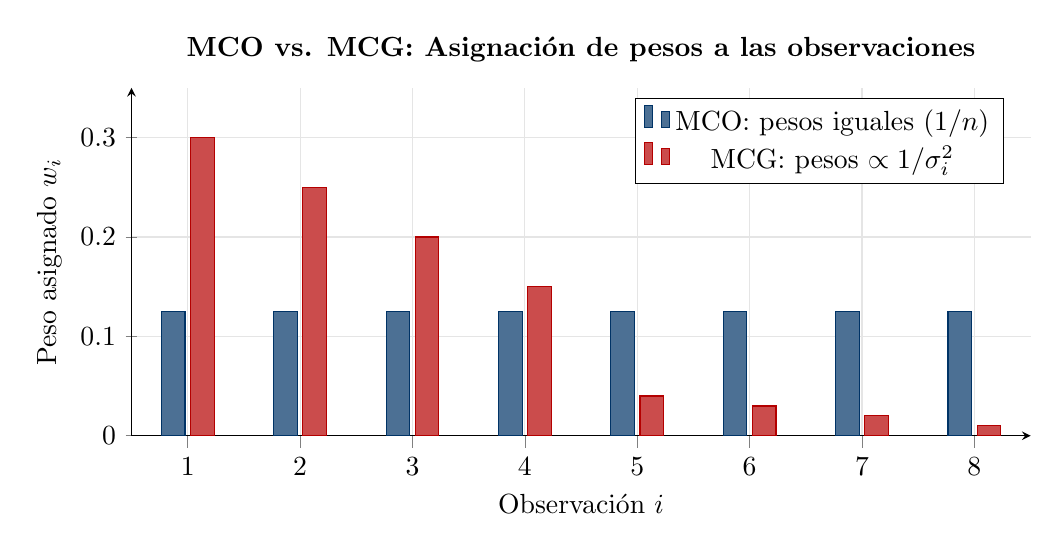
\begin{tikzpicture}
    \begin{axis}[
      width=13cm, height=6cm,
      xlabel={Observación $i$},
      ylabel={Peso asignado $w_i$},
      title={\textbf{MCO vs. MCG: Asignación de pesos a las observaciones}},
      xmin=0.5, xmax=8.5, ymin=0, ymax=0.35,
      xtick={1,2,3,4,5,6,7,8},
      xticklabels={1,2,3,4,5,6,7,8},
      legend pos=north east,
      grid=major, grid style={gray!20},
      axis lines=left,
      ybar,
      bar width=0.3cm,
    ]
      \addplot[fill=azuloscuro!70, draw=azuloscuro] coordinates {
        (1,0.125)(2,0.125)(3,0.125)(4,0.125)(5,0.125)(6,0.125)(7,0.125)(8,0.125)
      };
      \addlegendentry{MCO: pesos iguales ($1/n$)}
      \addplot[fill=rojoalerta!70, draw=rojoalerta] coordinates {
        (1,0.30)(2,0.25)(3,0.20)(4,0.15)(5,0.04)(6,0.03)(7,0.02)(8,0.01)
      };
      \addlegendentry{MCG: pesos $\propto 1/\sigma_i^2$}
    \end{axis}
  \end{tikzpicture}
  \caption{Comparación de la asignación de pesos entre MCO y MCG. MCO asigna el mismo peso $1/n$ a todas las observaciones sin importar su variabilidad. MCG asigna mayores pesos a las observaciones de menor varianza (más informativas), siendo más eficiente.}
  \label{fig:pesos_mco_mcg}
\end{figure}

\section{Mínimos Cuadrados Generalizados (MCG)}

\subsection{Fundamento y Lógica de la Transformación}

El \textbf{Método de Mínimos Cuadrados Generalizados} (MCG) fue propuesto por Aitken (1935) y constituye la solución óptima al problema de estimación bajo una estructura de perturbaciones no esféricas. La idea central es \textit{transformar} el modelo para que los errores transformados sí cumplan los supuestos del MLC.

\subsubsection{Modelo Original (Heteroscedástico)}

\begin{equation}
  Y_i = \beta_1 + \beta_2 X_i + u_i, \qquad \E(u_i^2) = \sigma_i^2
  \label{eq:modelo_original}
\end{equation}

\subsubsection{Transformación de Varianza Estabilizadora}

Si las varianzas $\sigma_i^2$ son conocidas, dividir cada término de la ecuación por $\sigma_i$:
\begin{equation}
  \underbrace{\frac{Y_i}{\sigma_i}}_{Y_i^*} = \beta_1 \underbrace{\frac{1}{\sigma_i}}_{X_{0i}^*} + \beta_2 \underbrace{\frac{X_i}{\sigma_i}}_{X_i^*} + \underbrace{\frac{u_i}{\sigma_i}}_{u_i^*}
  \label{eq:modelo_transformado}
\end{equation}

Verificando la homocedasticidad del modelo transformado:
\begin{equation}
  \E\left[(u_i^*)^2\right] = \E\left[\left(\frac{u_i}{\sigma_i}\right)^2\right] = \frac{1}{\sigma_i^2}\E(u_i^2) = \frac{\sigma_i^2}{\sigma_i^2} = 1
  \label{eq:verif_homo}
\end{equation}

Por lo tanto, $u_i^* \sim (0, 1)$: el modelo transformado \eqref{eq:modelo_transformado} satisface el supuesto de homocedasticidad y puede estimarse eficientemente por MCO.

\begin{tcolorbox}[notastyle, title={Nota Importante: Pérdida del Intercepto}]
  Nótese que en el modelo transformado \eqref{eq:modelo_transformado}, la ``constante'' ya no es un escalar sino la variable $1/\sigma_i$, que varía entre observaciones. Por ello, la regresión transformada \textbf{no tiene intercepto convencional}, sino que $\beta_1$ se estima como el coeficiente de la variable $1/\sigma_i$. El investigador debe ser cuidadoso con los grados de libertad y la interpretación del $R^2$.
\end{tcolorbox}

\subsection{Formulación Matricial General}

Matricialmente, el modelo es $\mathbf{y} = \mathbf{X}\boldsymbol{\beta} + \mathbf{u}$, donde $\E(\mathbf{u}\mathbf{u}') = \boldsymbol{\Omega}$. Sea $\boldsymbol{\Omega}^{-1/2}$ la raíz cuadrada inversa de $\boldsymbol{\Omega}$ (existe dado que $\boldsymbol{\Omega}$ es definida positiva). Pre-multiplicar por $\boldsymbol{\Omega}^{-1/2}$:
\begin{equation}
  \underbrace{\boldsymbol{\Omega}^{-1/2}\mathbf{y}}_{\mathbf{y}^*} = \underbrace{\boldsymbol{\Omega}^{-1/2}\mathbf{X}}_{\mathbf{X}^*}\boldsymbol{\beta} + \underbrace{\boldsymbol{\Omega}^{-1/2}\mathbf{u}}_{\mathbf{u}^*}
  \label{eq:modelo_matricial_trans}
\end{equation}

La varianza del error transformado es:
\begin{equation}
  \E(\mathbf{u}^*\mathbf{u}^{*'}) = \boldsymbol{\Omega}^{-1/2}\E(\mathbf{u}\mathbf{u}')\boldsymbol{\Omega}^{-1/2} = \boldsymbol{\Omega}^{-1/2}\boldsymbol{\Omega}\boldsymbol{\Omega}^{-1/2} = \mathbf{I}_n
  \label{eq:var_u_star}
\end{equation}

Aplicando MCO al modelo transformado:
\begin{equation}
  \boxed{
  \betahat_{\GLS} = (\mathbf{X}^{*'}\mathbf{X}^*)^{-1}\mathbf{X}^{*'}\mathbf{y}^* = (\mathbf{X}'\boldsymbol{\Omega}^{-1}\mathbf{X})^{-1}\mathbf{X}'\boldsymbol{\Omega}^{-1}\mathbf{y}
  }
  \label{eq:gls_estimator}
\end{equation}

La varianza de este estimador es:
\begin{equation}
  \Var(\betahat_{\GLS}) = (\mathbf{X}'\boldsymbol{\Omega}^{-1}\mathbf{X})^{-1}
  \label{eq:var_gls}
\end{equation}

\begin{tcolorbox}[teoremastyle, title={Teorema de Aitken (Gauss-Markov Generalizado)}]
  \textbf{Enunciado:} Bajo el modelo $\mathbf{y} = \mathbf{X}\boldsymbol{\beta} + \mathbf{u}$ con $\E(\mathbf{u}) = \mathbf{0}$ y $\E(\mathbf{u}\mathbf{u}') = \boldsymbol{\Omega}$ (conocida), el estimador MCG definido en \eqref{eq:gls_estimator} es el \textbf{Mejor Estimador Lineal Insesgado (BLUE)}.

  \textbf{Demostración (Sketch):} Sea $\tilde{\boldsymbol{\beta}} = \mathbf{C}\mathbf{y}$ cualquier estimador lineal insesgado alternativo. La condición de insesgadez requiere $\mathbf{C}\mathbf{X} = \mathbf{I}$. Sea $\mathbf{D} = \mathbf{C} - (\mathbf{X}'\boldsymbol{\Omega}^{-1}\mathbf{X})^{-1}\mathbf{X}'\boldsymbol{\Omega}^{-1}$. Entonces:
  \begin{align*}
    \Var(\tilde{\boldsymbol{\beta}}) - \Var(\betahat_{\GLS})
    &= \mathbf{C}\boldsymbol{\Omega}\mathbf{C}' - (\mathbf{X}'\boldsymbol{\Omega}^{-1}\mathbf{X})^{-1}\\
    &= \mathbf{D}\boldsymbol{\Omega}\mathbf{D}' \succeq \mathbf{0}
  \end{align*}
  puesto que $\mathbf{D}\boldsymbol{\Omega}\mathbf{D}'$ es semidefinida positiva. $\blacksquare$
\end{tcolorbox}

\subsection{Mínimos Cuadrados Ponderados (MCP)}

Cuando $\boldsymbol{\Omega}$ es diagonal (heteroscedasticidad pura sin autocorrelación), MCG se reduce a \textbf{Mínimos Cuadrados Ponderados}. El estimador minimiza la suma ponderada de cuadrados residuales:

\begin{equation}
  S^* = \sum_{i=1}^n w_i (Y_i - \beta_1 - \beta_2 X_i)^2, \qquad w_i = \frac{1}{\sigma_i^2}
  \label{eq:wls_obj}
\end{equation}

Las condiciones de primer orden conducen a:
\begin{align}
  \sum_{i=1}^n w_i (Y_i - \betahat_1^* - \betahat_2^* X_i) &= 0 \label{eq:wls_cpo1}\\
  \sum_{i=1}^n w_i X_i (Y_i - \betahat_1^* - \betahat_2^* X_i) &= 0 \label{eq:wls_cpo2}
\end{align}

De donde el estimador MCP de la pendiente es:
\begin{equation}
  \betahat_2^* = \frac{\sum w_i x_i y_i}{\sum w_i x_i^2}
  \label{eq:wls_slope}
\end{equation}
con $x_i = X_i - \bar{X}_w$ y $\bar{X}_w = \frac{\sum w_i X_i}{\sum w_i}$ siendo la media ponderada de $X$.

\begin{figure}[H]
  \centering
  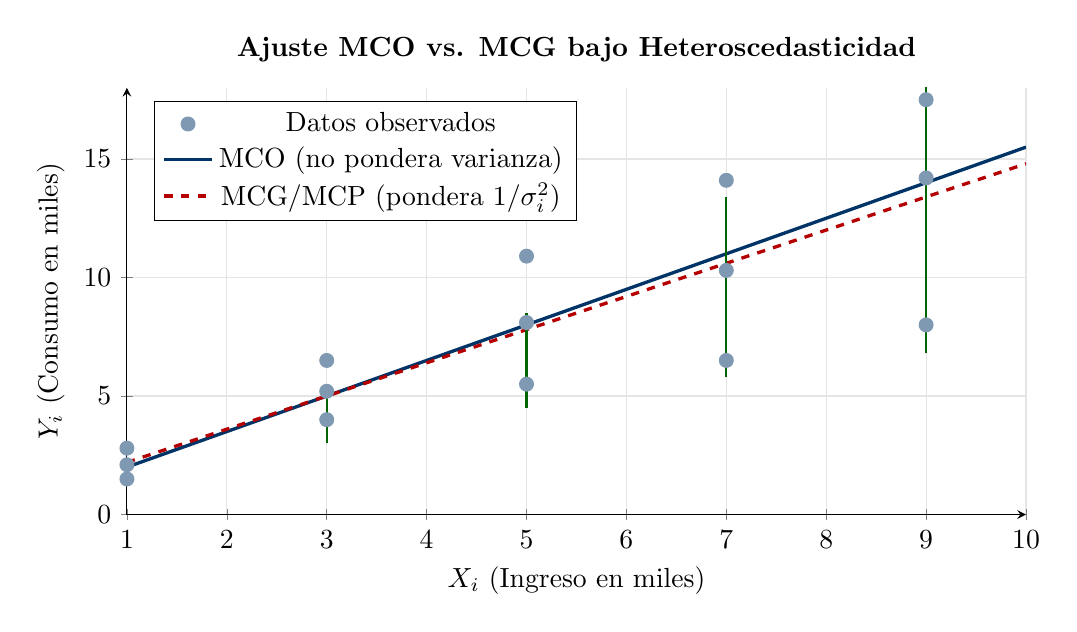
\begin{tikzpicture}
    \begin{axis}[
      width=13cm, height=7cm,
      xlabel={$X_i$ (Ingreso en miles)},
      ylabel={$Y_i$ (Consumo en miles)},
      title={\textbf{Ajuste MCO vs. MCG bajo Heteroscedasticidad}},
      xmin=1, xmax=10, ymin=0, ymax=18,
      legend pos=north west,
      grid=major, grid style={gray!20},
      axis lines=left,
    ]
      \addplot[only marks, mark=*, mark size=2.5pt, color=azuloscuro!50]
        coordinates {
          (1,2.1)(1,1.5)(1,2.8)
          (3,5.2)(3,4.0)(3,6.5)
          (5,8.1)(5,5.5)(5,10.9)
          (7,10.3)(7,6.5)(7,14.1)
          (9,14.2)(9,8.0)(9,17.5)
        };
      \addplot[azuloscuro, very thick, domain=1:10] {1.5*x + 0.5};
      \addlegendentry{Datos observados}
      \addlegendentry{MCO (no pondera varianza)}
      \addplot[rojoalerta, very thick, dashed, domain=1:10] {1.4*x + 0.8};
      \addlegendentry{MCG/MCP (pondera $1/\sigma_i^2$)}
      \addplot[verdematematica, thick] coordinates {(1,1.4)(1,2.2)};
      \addplot[verdematematica, thick] coordinates {(3,3.0)(3,5.0)};
      \addplot[verdematematica, thick] coordinates {(5,4.5)(5,8.5)};
      \addplot[verdematematica, thick] coordinates {(7,5.8)(7,13.4)};
      \addplot[verdematematica, thick] coordinates {(9,6.8)(9,18.4)};
    \end{axis}
  \end{tikzpicture}
  \caption{MCO y MCG producen líneas similares, pero MCG pondera cada observación inversamente proporcional a su varianza $\sigma_i^2$. Las barras verdes representan la dispersión condicional de cada grupo.}
  \label{fig:mco_vs_mcg}
\end{figure}

\subsection{El Problema Práctico: Varianzas Desconocidas}

En la práctica, $\sigma_i^2$ no se conoce. Las soluciones son:

\begin{enumerate}[label=\textbf{Opción \arabic*:}]
  \item \textbf{MCG Factible (FGLS):} Estimar $\sigma_i^2$ a partir de los residuales de una primera regresión MCO, ajustando un modelo para la varianza (ej. Park) y usar las varianzas estimadas como pesos.
  \item \textbf{Errores Estándar Robustos (White):} Mantener el estimador MCO pero corregir la matriz de varianza-covarianza usando el estimador de White.
  \item \textbf{Transformaciones ad hoc:} Si se sospecha que $\sigma_i^2 \propto X_i^2$, dividir por $X_i$; si $\sigma_i^2 \propto X_i$, dividir por $\sqrt{X_i}$.
\end{enumerate}

\section{Consecuencias Formales del Uso de MCO}

\subsection{Resumen de Propiedades}

\begin{table}[H]
  \centering
  \caption{Propiedades del estimador MCO bajo homocedasticidad vs. heteroscedasticidad}
  \label{tab:propiedades}
  \begin{tabular}{lccc}
    \toprule
    \textbf{Propiedad} & \textbf{Condición} & \textbf{Bajo Homo.} & \textbf{Bajo Hetero.} \\
    \midrule
    Lineal & Siempre & \checkmark & \checkmark \\
    Insesgado & Exogeneidad & \checkmark & \checkmark \\
    Consistente & Exog. + regulares & \checkmark & \checkmark \\
    Eficiente (BLUE) & Gauss-Markov & \checkmark & \textbf{NO} \\
    Var. correcta & Homocedasticidad & \checkmark & \textbf{NO} \\
    Pruebas $t$/$F$ válidas & Var. correcta & \checkmark & \textbf{NO} \\
    Intervalos conf. válidos & Var. correcta & \checkmark & \textbf{NO} \\
    \bottomrule
  \end{tabular}
\end{table}

\subsection{El Sesgo en el Estimador de la Varianza}

El estimador habitual de $\sigma^2$ es:
\begin{equation}
  \sigmahat^2 = \frac{\sum_{i=1}^n \uhat_i^2}{n - k} = \frac{\mathbf{u}'\mathbf{M}\mathbf{u}}{n - k}
  \label{eq:sigma2_hat}
\end{equation}
donde $\mathbf{M} = \mathbf{I} - \mathbf{X}(\mathbf{X}'\mathbf{X})^{-1}\mathbf{X}'$ es la matriz de proyección ortogonal.

Bajo heteroscedasticidad:
\begin{align}
  \E(\sigmahat^2) &= \frac{1}{n-k}\E(\mathbf{u}'\mathbf{M}\mathbf{u}) = \frac{1}{n-k}\mathrm{tr}(\mathbf{M}\boldsymbol{\Omega})
  \label{eq:e_sigma2}
\end{align}

Mientras que si hubiera homocedasticidad: $\frac{1}{n-k}\mathrm{tr}(\mathbf{M}\sigma^2\mathbf{I}) = \sigma^2$. Con heteroscedasticidad, $\mathrm{tr}(\mathbf{M}\boldsymbol{\Omega}) \neq (n-k)\sigma^2$, por lo que $\sigmahat^2$ es un estimador \textbf{sesgado}.

\subsection{Consecuencias en las Pruebas de Hipótesis}

\begin{tcolorbox}[alertastyle, title={Invalidez de las Pruebas $t$ y $F$}]
  \textbf{Estadístico $t$ convencional:}
  \begin{equation}
    t_j = \frac{\betahat_j - \beta_j^0}{\widehat{\text{se}}(\betahat_j)}
    \label{eq:t_stat}
  \end{equation}
  donde $\widehat{\text{se}}(\betahat_j) = \sqrt{\sigmahat^2 [(\mathbf{X}'\mathbf{X})^{-1}]_{jj}}$.

  Bajo heteroscedasticidad, el numerador tiene distribución normal correcta (insesgadez), pero el denominador es incorrecto. Por tanto, $t_j$ \textbf{no sigue una distribución $t$ de Student} con $n-k$ grados de libertad. Las conclusiones sobre significancia estadística son inválidas.

  \textbf{Consecuencias prácticas:}
  \begin{itemize}
    \item Si $\widehat{\text{se}}$ subestima el verdadero error estándar $\Rightarrow$ el estadístico $t$ está inflado $\Rightarrow$ se \textbf{rechaza $H_0$ con demasiada frecuencia} (tamaño real $>$ nivel nominal $\alpha$).
    \item Si $\widehat{\text{se}}$ sobreestima el verdadero error estándar $\Rightarrow$ el estadístico $t$ está desinflado $\Rightarrow$ se \textbf{acepta $H_0$ erróneamente} (pérdida de potencia).
  \end{itemize}
\end{tcolorbox}

\section{Detección de la Heteroscedasticidad}

\subsection{Métodos Gráficos}

\begin{tcolorbox}[notastyle, title={Procedimiento Gráfico}]
  \begin{enumerate}[label=\textbf{Paso \arabic*:}]
    \item Estimar el modelo por MCO y obtener los residuales $\uhat_i$.
    \item Graficar $\uhat_i$ (o $\uhat_i^2$) vs. $\yhat_i$ (valores ajustados) o vs. las variables explicativas $X_j$.
    \item Si el gráfico muestra un patrón sistemático (embudo, forma cuadrática, etc.), esto sugiere heteroscedasticidad. Si los puntos se dispersan aleatoriamente, no hay evidencia.
  \end{enumerate}
\end{tcolorbox}

\begin{figure}[H]
  \centering
  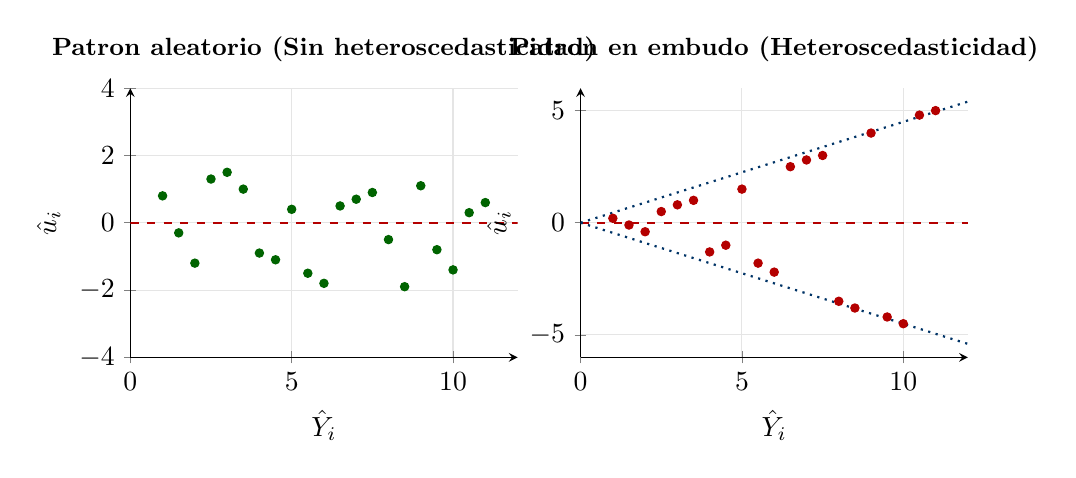
\begin{tikzpicture}
    \begin{axis}[
      name=g1,
      width=6.5cm, height=5cm,
      xlabel={$\hat{Y}_i$}, ylabel={$\hat{u}_i$},
      title={\small\textbf{Patron aleatorio (Sin heteroscedasticidad)}},
      xmin=0, xmax=12, ymin=-4, ymax=4,
      grid=major, grid style={gray!20}, axis lines=left,
    ]
      \addplot[only marks, mark=*, mark size=1.5pt, color=verdematematica]
        coordinates {
          (1,0.8)(2,-1.2)(3,1.5)(4,-0.9)(5,0.4)(6,-1.8)(7,0.7)(8,-0.5)
          (9,1.1)(10,-1.4)(11,0.6)(1.5,-0.3)(3.5,1.0)(5.5,-1.5)(7.5,0.9)(9.5,-0.8)
          (2.5,1.3)(4.5,-1.1)(6.5,0.5)(8.5,-1.9)(10.5,0.3)
        };
      \addplot[rojoalerta, thick, dashed, domain=0:12] {0};
    \end{axis}

    \begin{axis}[
      name=g2,
      at={(g1.east)}, anchor=west, xshift=0.8cm,
      width=6.5cm, height=5cm,
      xlabel={$\hat{Y}_i$}, ylabel={$\hat{u}_i$},
      title={\small\textbf{Patron en embudo (Heteroscedasticidad)}},
      xmin=0, xmax=12, ymin=-6, ymax=6,
      grid=major, grid style={gray!20}, axis lines=left,
    ]
      \addplot[only marks, mark=*, mark size=1.5pt, color=rojoalerta]
        coordinates {
          (1,0.2)(2,-0.4)(3,0.8)(4,-1.3)(5,1.5)(6,-2.2)(7,2.8)(8,-3.5)
          (9,4.0)(10,-4.5)(11,5.0)(1.5,-0.1)(3.5,1.0)(5.5,-1.8)(7.5,3.0)(9.5,-4.2)
          (2.5,0.5)(4.5,-1.0)(6.5,2.5)(8.5,-3.8)(10.5,4.8)
        };
      \addplot[rojoalerta, thick, dashed, domain=0:12] {0};
      \addplot[azuloscuro, thick, dotted, domain=0:12] {0.45*x};
      \addplot[azuloscuro, thick, dotted, domain=0:12] {-0.45*x};
    \end{axis}
  \end{tikzpicture}
  \caption{Gráficos de residuales vs. valores ajustados. El panel izquierdo muestra dispersión aleatoria (homocedasticidad). El panel derecho muestra el patrón típico en ``embudo'' de la heteroscedasticidad, donde la dispersión aumenta con $\hat{Y}_i$.}
  \label{fig:residual_plots}
\end{figure}

\subsection{Prueba de Park}

Park (1966) propuso modelar la varianza como una función potencial de una variable explicativa:
\begin{equation}
  \sigma_i^2 = \sigma^2 X_i^{\delta} e^{v_i}
  \label{eq:park_model}
\end{equation}

Tomando logaritmos:
\begin{equation}
  \ln(\sigma_i^2) = \ln(\sigma^2) + \delta \ln(X_i) + v_i
  \label{eq:park_log}
\end{equation}

Como $\sigma_i^2$ no es observable, se aproxima con $\uhat_i^2$ de la regresión MCO:
\begin{equation}
  \ln(\uhat_i^2) = \alpha_0 + \delta \ln(X_i) + v_i
  \label{eq:park_regresion}
\end{equation}

\textbf{Decisión:} Si $\delta$ es estadísticamente significativo (prueba $t$), existe evidencia de heteroscedasticidad. La limitación es que $v_i$ puede no ser bien comportado.

\subsection{Prueba de Glejser}

Glejser (1969) propone regresar el valor absoluto de los residuales sobre las variables explicativas bajo diferentes formas funcionales:

\begin{align}
  |\uhat_i| &= \alpha_0 + \alpha_1 X_i + v_i \label{eq:glejser1}\\
  |\uhat_i| &= \alpha_0 + \alpha_1 \sqrt{X_i} + v_i \label{eq:glejser2}\\
  |\uhat_i| &= \alpha_0 + \alpha_1 / X_i + v_i \label{eq:glejser3}\\
  |\uhat_i| &= \alpha_0 + \alpha_1 / \sqrt{X_i} + v_i \label{eq:glejser4}
\end{align}

\textbf{Decisión:} Si $\alpha_1 \neq 0$ significativamente en alguna especificación, hay heteroscedasticidad.

\subsection{Prueba de Correlación de Rangos de Spearman}

\begin{tcolorbox}[notastyle, title={Procedimiento: Correlación de Spearman}]
  \begin{enumerate}[label=\textbf{Paso \arabic*:}]
    \item Estimar el modelo y obtener $|\uhat_i|$.
    \item Ordenar $|\uhat_i|$ y $X_i$ de menor a mayor, asignando rangos $d_{1i}$ y $d_{2i}$.
    \item Calcular las diferencias $d_i = d_{1i} - d_{2i}$.
    \item Computar el coeficiente de correlación de rangos:
    \begin{equation}
      r_s = 1 - \frac{6\sum_{i=1}^n d_i^2}{n(n^2 - 1)}
      \label{eq:spearman}
    \end{equation}
    \item Bajo $H_0$: no hay heteroscedasticidad, el estadístico:
    \begin{equation}
      t = \frac{r_s \sqrt{n-2}}{\sqrt{1-r_s^2}} \sim t_{n-2}
      \label{eq:spearman_t}
    \end{equation}
  \end{enumerate}
  Si $|t| > t_{\alpha/2, n-2}$, se rechaza $H_0$.
\end{tcolorbox}

\subsection{Prueba de Goldfeld-Quandt}

Diseñada para detectar si la varianza aumenta (o disminuye) con una variable ordenadora $X$:

\begin{tcolorbox}[notastyle, title={Procedimiento: Goldfeld-Quandt}]
  \begin{enumerate}[label=\textbf{Paso \arabic*:}]
    \item Ordenar las $n$ observaciones según la variable explicativa sospechosa $X_i$.
    \item Eliminar las $c$ observaciones centrales (generalmente $c \approx n/5$).
    \item Dividir las $n - c$ observaciones restantes en dos grupos: $n_1 = n_2 = (n-c)/2$.
    \item Regresar el modelo por MCO en cada grupo, obteniendo $\text{RSS}_1$ y $\text{RSS}_2$ (con $\text{RSS}_2$ del grupo de mayor $X$).
    \item Calcular el estadístico:
    \begin{equation}
      F_{GQ} = \frac{\text{RSS}_2 / (n_2 - k)}{\text{RSS}_1 / (n_1 - k)} \sim F_{(n_2 - k), (n_1 - k)}
      \label{eq:gq_stat}
    \end{equation}
    \item Si $F_{GQ} > F_{\alpha, (n_2-k), (n_1-k)}$, rechazar $H_0$ (homocedasticidad).
  \end{enumerate}
\end{tcolorbox}

\begin{figure}[H]
  \centering
  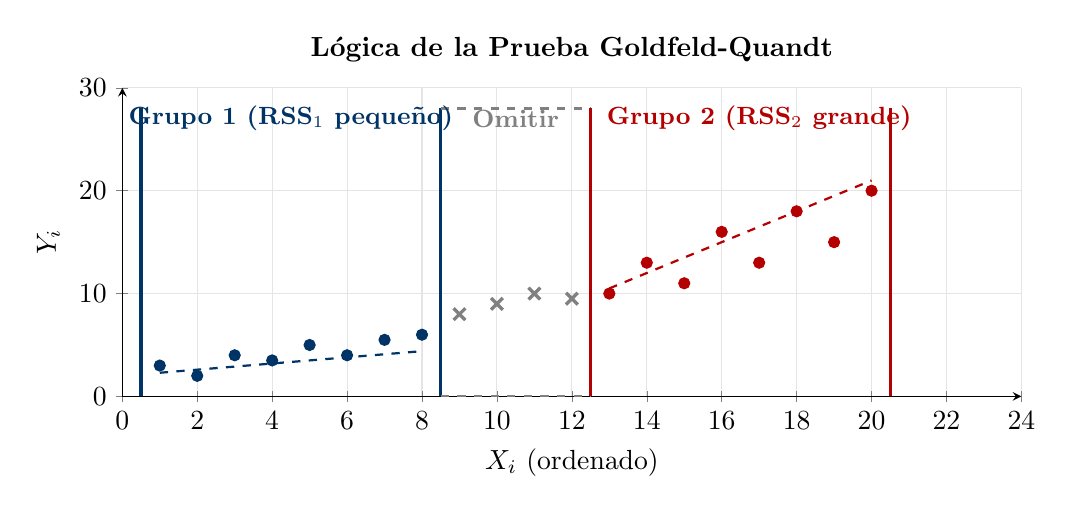
\begin{tikzpicture}
    \begin{axis}[
      width=13cm, height=5.5cm,
      xlabel={$X_i$ (ordenado)},
      ylabel={$Y_i$},
      title={\textbf{Lógica de la Prueba Goldfeld-Quandt}},
      xmin=0, xmax=24, ymin=0, ymax=30,
      axis lines=left,
      grid=major, grid style={gray!20},
    ]
      \addplot[only marks, mark=*, mark size=2pt, color=azuloscuro]
        coordinates {(1,3)(2,2)(3,4)(4,3.5)(5,5)(6,4)(7,5.5)(8,6)};
      \addplot[only marks, mark=x, mark size=3pt, very thick, color=gray]
        coordinates {(9,8)(10,9)(11,10)(12,9.5)};
      \addplot[only marks, mark=*, mark size=2pt, color=rojoalerta]
        coordinates {(13,10)(14,13)(15,11)(16,16)(17,13)(18,18)(19,15)(20,20)};

      \draw[azuloscuro, very thick] (axis cs:0.5,0) -- (axis cs:0.5,28);
      \draw[azuloscuro, very thick] (axis cs:8.5,0) -- (axis cs:8.5,28);
      \draw[gray, very thick, dashed] (axis cs:8.5,0) -- (axis cs:12.5,0);
      \draw[gray, very thick, dashed] (axis cs:8.5,28) -- (axis cs:12.5,28);
      \draw[gray, very thick] (axis cs:12.5,0) -- (axis cs:12.5,28);
      \draw[rojoalerta, very thick] (axis cs:12.5,0) -- (axis cs:12.5,28);
      \draw[rojoalerta, very thick] (axis cs:20.5,0) -- (axis cs:20.5,28);

      \node[azuloscuro, font=\small\bfseries] at (axis cs:4.5,27) {Grupo 1 ($\text{RSS}_1$ pequeño)};
      \node[gray, font=\small\bfseries] at (axis cs:10.5,27) {Omitir};
      \node[rojoalerta, font=\small\bfseries] at (axis cs:17,27) {Grupo 2 ($\text{RSS}_2$ grande)};

      \addplot[azuloscuro, thick, dashed, domain=1:8] {0.3*x + 2};
      \addplot[rojoalerta, thick, dashed, domain=13:20] {1.5*x - 9};
    \end{axis}
  \end{tikzpicture}
  \caption{Ilustración de la prueba Goldfeld-Quandt. Las observaciones se ordenan por $X$, se elimina el grupo central y se compara la varianza residual entre los grupos extremos. Si $\text{RSS}_2 \gg \text{RSS}_1$, la varianza crece con $X$.}
  \label{fig:gq}
\end{figure}

\subsection{Prueba de Breusch-Pagan-Godfrey (BPG)}

Breusch y Pagan (1979), y Godfrey (1978) de forma independiente, propusieron una prueba de multiplicadores de Lagrange (LM).

\textbf{Supuesto:} $\sigma_i^2 = f(\alpha_0 + \alpha_1 Z_{1i} + \cdots + \alpha_p Z_{pi})$, donde $Z_{ji}$ son variables que supuestamente causan la heteroscedasticidad.

$H_0: \alpha_1 = \alpha_2 = \cdots = \alpha_p = 0$ (homocedasticidad).

\begin{tcolorbox}[notastyle, title={Procedimiento: Breusch-Pagan-Godfrey}]
  \begin{enumerate}[label=\textbf{Paso \arabic*:}]
    \item Estimar el modelo por MCO. Obtener $\uhat_i$ y $\sigmahat^2 = \sum \uhat_i^2/n$.
    \item Construir la variable:
    \begin{equation}
      p_i = \frac{\uhat_i^2}{\sigmahat^2}
      \label{eq:bpg_pi}
    \end{equation}
    \item Regresar $p_i$ sobre las variables $Z_{ji}$:
    \begin{equation}
      p_i = \alpha_0 + \alpha_1 Z_{1i} + \cdots + \alpha_p Z_{pi} + \varepsilon_i
      \label{eq:bpg_regresion}
    \end{equation}
    \item Calcular la suma de cuadrados explicada (SCE) de esta regresión auxiliar.
    \item El estadístico LM:
    \begin{equation}
      \chi^2_{BPG} = \frac{\text{SCE}}{2} \xrightarrow{d} \chi^2_{(p)}
      \label{eq:bpg_stat}
    \end{equation}
  \end{enumerate}
\end{tcolorbox}

\subsection{Prueba de White}

White (1980) propuso una prueba más general que no requiere especificar la forma de la heteroscedasticidad.

\begin{tcolorbox}[notastyle, title={Procedimiento: Prueba de White}]
  \begin{enumerate}[label=\textbf{Paso \arabic*:}]
    \item Estimar el modelo original por MCO. Obtener $\uhat_i$.
    \item Regresar $\uhat_i^2$ sobre todos los regresores originales, sus cuadrados y productos cruzados. Para el modelo $Y = \beta_1 + \beta_2 X_2 + \beta_3 X_3 + u$:
    \begin{equation}
      \uhat_i^2 = \alpha_0 + \alpha_1 X_{2i} + \alpha_2 X_{3i} + \alpha_3 X_{2i}^2 + \alpha_4 X_{3i}^2 + \alpha_5 X_{2i}X_{3i} + v_i
      \label{eq:white_regresion}
    \end{equation}
    \item El estadístico de White:
    \begin{equation}
      W = n \cdot R_{\text{aux}}^2 \xrightarrow{d} \chi^2_{(p)}
      \label{eq:white_stat}
    \end{equation}
    donde $p$ es el número de regresores en \eqref{eq:white_regresion} (excluida la constante).
    \item Rechazar $H_0$ si $W > \chi^2_{\alpha, p}$.
  \end{enumerate}
\end{tcolorbox}

\textbf{Versión simplificada (Davidson-MacKinnon):} Una alternativa es regresar $\uhat_i^2$ sobre $\yhat_i$ y $\yhat_i^2$:
\begin{equation}
  \uhat_i^2 = \delta_0 + \delta_1 \yhat_i + \delta_2 \yhat_i^2 + v_i
  \label{eq:white_simple}
\end{equation}
y usar $n \cdot R^2$ de esta regresión como estadístico $\chi^2_{(2)}$.

\begin{figure}[H]
  \centering
  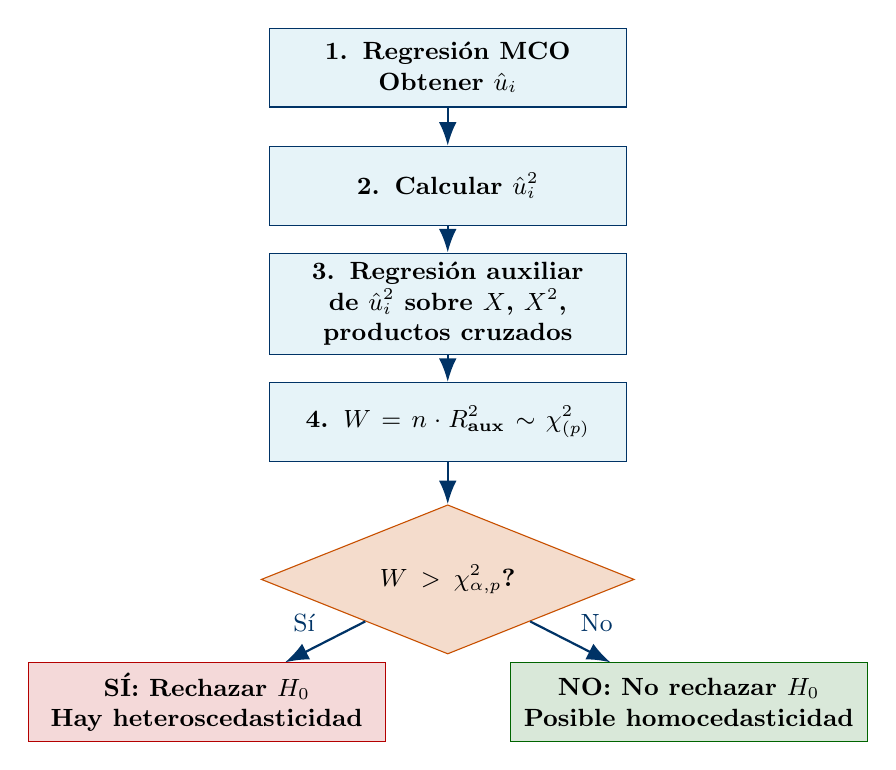
\begin{tikzpicture}[node distance=1.5cm, auto,
    box/.style={rectangle, draw=azuloscuro, fill=azulclaro!30,
                minimum width=4.5cm, minimum height=1cm,
                text centered, font=\small\bfseries, text width=4.3cm},
    decision/.style={diamond, draw=naranjaejemplo, fill=naranjaejemplo!20,
                     minimum width=3.5cm, minimum height=1.2cm,
                     text centered, font=\small\bfseries, text width=3cm,
                     aspect=2.5},
    arrow/.style={-{Latex[length=3mm]}, thick, color=azuloscuro}
  ]
    \node[box] (paso1) {1. Regresión MCO\\Obtener $\uhat_i$};
    \node[box, below of=paso1] (paso2) {2. Calcular $\uhat_i^2$};
    \node[box, below of=paso2] (paso3) {3. Regresión auxiliar de $\uhat_i^2$ sobre $X$, $X^2$, productos cruzados};
    \node[box, below of=paso3] (paso4) {4. $W = n \cdot R^2_{\text{aux}} \sim \chi^2_{(p)}$};
    \node[decision, below of=paso4, yshift=-0.5cm] (decision) {$W > \chi^2_{\alpha,p}$?};
    \node[box, below left of=decision, xshift=-2cm, yshift=-0.5cm,
          draw=rojoalerta, fill=rojoalerta!15] (si) {SÍ: Rechazar $H_0$\\Hay heteroscedasticidad};
    \node[box, below right of=decision, xshift=2cm, yshift=-0.5cm,
          draw=verdematematica, fill=verdematematica!15] (no) {NO: No rechazar $H_0$\\Posible homocedasticidad};

    \draw[arrow] (paso1) -- (paso2);
    \draw[arrow] (paso2) -- (paso3);
    \draw[arrow] (paso3) -- (paso4);
    \draw[arrow] (paso4) -- (decision);
    \draw[arrow] (decision) -- node[above left, font=\small]{Sí} (si);
    \draw[arrow] (decision) -- node[above right, font=\small]{No} (no);
  \end{tikzpicture}
  \caption{Diagrama de flujo de la Prueba de White para heteroscedasticidad.}
  \label{fig:white_flowchart}
\end{figure}

\section{Medidas Remediales}

\subsection{Cuando se Conoce $\sigma_i^2$: Mínimos Cuadrados Ponderados Exactos}

Si se conoce la forma exacta de la heteroscedasticidad, se aplica MCP con $w_i = 1/\sigma_i^2$. Algunos casos especiales:

\begin{table}[H]
  \centering
  \caption{Transformaciones MCP según la forma de $\sigma_i^2$}
  \label{tab:transformaciones}
  \begin{tabular}{lll}
    \toprule
    \textbf{Supuesto sobre $\sigma_i^2$} & \textbf{Transformación} & \textbf{Modelo transformado} \\
    \midrule
    $\sigma_i^2 = \sigma^2 X_i^2$ & Dividir por $X_i$ & $Y_i/X_i = \beta_1/X_i + \beta_2 + u_i/X_i$ \\
    $\sigma_i^2 = \sigma^2 X_i$ & Dividir por $\sqrt{X_i}$ & $Y_i/\sqrt{X_i} = \beta_1/\sqrt{X_i} + \beta_2\sqrt{X_i} + u_i/\sqrt{X_i}$ \\
    $\sigma_i^2 = \sigma^2 E(Y_i)^2$ & Dividir por $\hat{Y}_i$ & $Y_i/\hat{Y}_i = \beta_1/\hat{Y}_i + \beta_2 X_i/\hat{Y}_i + u_i/\hat{Y}_i$ \\
    $\sigma_i^2 = \sigma^2 / n_i$ (grupos) & Multiplicar por $\sqrt{n_i}$ & Usar promedios de grupo \\
    \bottomrule
  \end{tabular}
\end{table}

\subsection{Errores Estándar Robustos de White (HC)}

Cuando la forma de $\boldsymbol{\Omega}$ es desconocida pero la muestra es grande, White (1980) propuso el estimador consistente de la varianza-covarianza:

\begin{equation}
  \widehat{\Var}_{\text{White}}(\betahat_{\OLS}) = (\mathbf{X}'\mathbf{X})^{-1} \left(\sum_{i=1}^n \uhat_i^2 \mathbf{x}_i \mathbf{x}_i'\right) (\mathbf{X}'\mathbf{X})^{-1}
  \label{eq:white_sandwich}
\end{equation}

donde $\mathbf{x}_i$ es el vector de regresores de la observación $i$. Este estimador es consistente bajo heterocedasticidad de forma desconocida para muestras grandes ($n \to \infty$).

\begin{tcolorbox}[notastyle, title={Variantes del Estimador Robusto (HC0 a HC3)}]
  \begin{itemize}
    \item \textbf{HC0 (White):} $\uhat_i^2$ sin corrección. Puede tener sesgo en muestras pequeñas.
    \item \textbf{HC1:} $\uhat_i^2 \cdot n/(n-k)$. Corrección de grados de libertad.
    \item \textbf{HC2:} $\uhat_i^2/(1-h_{ii})$ donde $h_{ii}$ son los leverage. Corrige por influencia.
    \item \textbf{HC3:} $\uhat_i^2/(1-h_{ii})^2$. Mejor desempeño en muestras pequeñas (MacKinnon-White).
  \end{itemize}
\end{tcolorbox}

\subsection{Transformación Logarítmica}

Si $Y > 0$ y $X > 0$, la transformación log-log:
\begin{equation}
  \ln Y_i = \gamma_1 + \gamma_2 \ln X_i + v_i
  \label{eq:log_log}
\end{equation}
frecuentemente reduce la heteroscedasticidad, ya que el logaritmo comprime la escala de las variables, especialmente en el caso de distribuciones asimétricas.

\textbf{Justificación estadística:} Si $\sigma_i^2 \propto [E(Y_i)]^2$ (varianza proporcional al cuadrado de la media), entonces:
\begin{equation}
  \text{CV}(Y_i) = \frac{\sigma_i}{E(Y_i)} = \text{constante}
  \label{eq:cv_const}
\end{equation}

En este caso, la transformación logarítmica produce varianza aproximadamente constante, ya que $\Var(\ln Y_i) \approx \Var(Y_i)/[E(Y_i)]^2 = \text{CV}^2$.

\section{Ejemplos Finales con Datos Reales}

\subsection{Ejemplo 11.9: Mortalidad Infantil Revisitada}

Se considera el modelo de regresión múltiple para una muestra de 64 países:
\begin{equation}
  CM_i = \beta_1 + \beta_2 \text{PGNP}_i + \beta_3 \text{FLR}_i + u_i
  \label{eq:mortalidad}
\end{equation}
donde $CM$ = mortalidad infantil (por mil nacidos vivos), $\text{PGNP}$ = PNB per cápita, $\text{FLR}$ = tasa de alfabetización femenina.

\textbf{Resultados MCO:}
\begin{equation}
  \widehat{CM}_i = 263.64 - 0.0056\,\text{PGNP}_i - 2.2316\,\text{FLR}_i
  \label{eq:mortalidad_ols}
\end{equation}

\begin{tcolorbox}[ejemplostyle, title={Aplicación de Pruebas de Heteroscedasticidad}]
  \textbf{Prueba de Glejser:} Regresión de $|\uhat_i|$ sobre $\widehat{CM}_i$:
  \begin{align*}
    |\uhat_i| &= 14.28 + 0.22\,\widehat{CM}_i\\
    t_{\text{pendiente}} &= 1.26 \quad (p\text{-valor} > 0.10)
  \end{align*}
  \textbf{Conclusión:} El estadístico $t = 1.26$ no es significativo al 10\%. No hay evidencia de heteroscedasticidad en este modelo. MCO estándar es adecuado.

  \textbf{Interpretación económica:} La heterogeneidad entre países de distintos niveles de desarrollo podría generar heteroscedasticidad. Sin embargo, el modelo ya captura la variabilidad mediante las variables de ingreso y alfabetización. Las perturbaciones restantes son homogéneas.
\end{tcolorbox}

\begin{figure}[H]
  \centering
  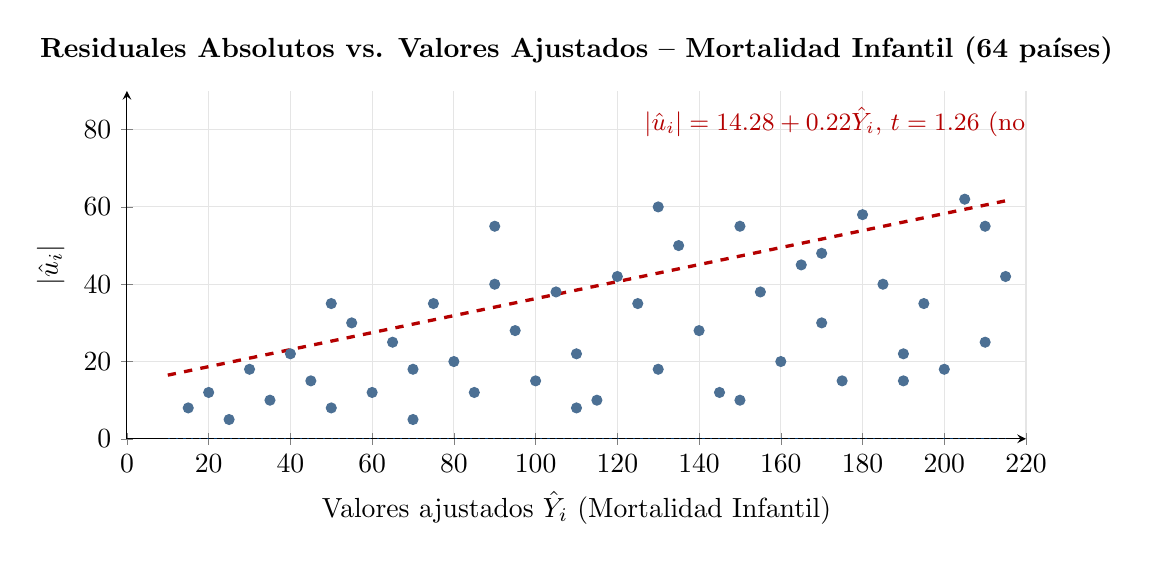
\begin{tikzpicture}
    \begin{axis}[
      width=13cm, height=6cm,
      xlabel={Valores ajustados $\hat{Y}_i$ (Mortalidad Infantil)},
      ylabel={$|\hat{u}_i|$},
      title={\textbf{Residuales Absolutos vs. Valores Ajustados -- Mortalidad Infantil (64 países)}},
      xmin=0, xmax=220, ymin=0, ymax=90,
      grid=major, grid style={gray!20},
      axis lines=left,
    ]
      \addplot[only marks, mark=*, mark size=1.8pt, color=azuloscuro!70]
        coordinates {
          (15,8)(20,12)(25,5)(30,18)(35,10)(40,22)(45,15)(50,8)
          (55,30)(60,12)(65,25)(70,18)(75,35)(80,20)(85,12)(90,40)
          (95,28)(100,15)(105,38)(110,22)(115,10)(120,42)(125,35)
          (130,18)(135,50)(140,28)(145,12)(150,55)(155,38)(160,20)
          (165,45)(170,30)(175,15)(180,58)(185,40)(190,22)(195,35)
          (200,18)(205,62)(210,25)(215,42)(50,35)(70,5)(90,55)
          (110,8)(130,60)(150,10)(170,48)(190,15)(210,55)
        };
      \addplot[rojoalerta, very thick, dashed, domain=10:215] {14.28 + 0.22*x};
      \addplot[azuloscuro, thick, dotted, domain=10:215] {0};
      \node[font=\small, color=rojoalerta] at (axis cs:180,82)
        {$|\hat{u}_i| = 14.28 + 0.22\hat{Y}_i$, $t=1.26$ (no sig.)};
    \end{axis}
  \end{tikzpicture}
  \caption{Gráfico de residuales absolutos vs. valores ajustados para el modelo de mortalidad infantil. La pendiente de la línea de tendencia no es estadísticamente significativa ($t = 1.26$), indicando ausencia de heteroscedasticidad.}
  \label{fig:mortalidad_residuales}
\end{figure}

\subsection{Ejemplo 11.10: Gasto en I+D -- Ventas y Utilidades}

Se analiza el gasto en Investigación y Desarrollo (I+D) para 18 grupos industriales:
\begin{equation}
  \text{I+D}_i = \beta_1 + \beta_2 \text{Ventas}_i + \beta_3 \text{Utilidades}_i + u_i
  \label{eq:id}
\end{equation}

\begin{figure}[H]
  \centering
  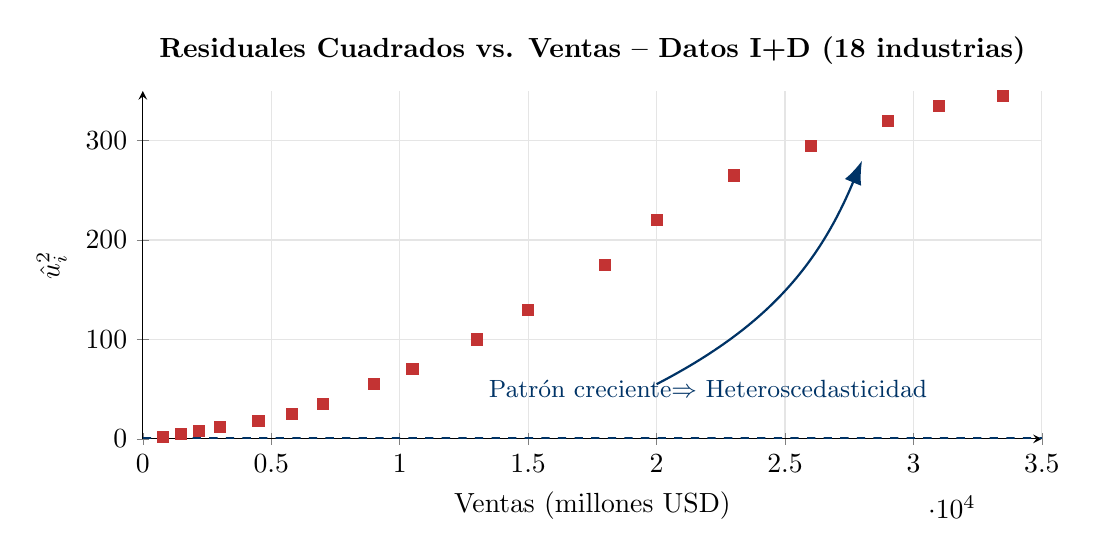
\begin{tikzpicture}
    \begin{axis}[
      width=13cm, height=6cm,
      xlabel={Ventas (millones USD)},
      ylabel={$\hat{u}_i^2$},
      title={\textbf{Residuales Cuadrados vs. Ventas -- Datos I+D (18 industrias)}},
      xmin=0, xmax=35000, ymin=0, ymax=350,
      grid=major, grid style={gray!20},
      axis lines=left,
    ]
      \addplot[only marks, mark=square*, mark size=2pt, color=rojoalerta!80]
        coordinates {
          (800,2)(1500,5)(2200,8)(3000,12)(4500,18)(5800,25)
          (7000,35)(9000,55)(10500,70)(13000,100)(15000,130)
          (18000,175)(20000,220)(23000,265)(26000,295)(29000,320)
          (31000,335)(33500,345)
        };
      \addplot[azuloscuro, very thick, dashed, domain=0:35000, samples=100]
        {0.00001*x^1.5/500};
      \node[font=\small, color=azuloscuro] at (axis cs:22000,50)
        {Patrón creciente$\Rightarrow$ Heteroscedasticidad};
      \draw[-{Latex[length=3mm]}, thick, azuloscuro] (axis cs:20000,55)
        to[bend right=20] (axis cs:28000,280);
    \end{axis}
  \end{tikzpicture}
  \caption{Los residuales cuadrados crecen sistemáticamente con el nivel de ventas, confirmando la presencia de heteroscedasticidad. Las grandes industrias tienen mayor variabilidad en el gasto de I+D.}
  \label{fig:id_residuales}
\end{figure}

\begin{tcolorbox}[ejemplostyle, title={Resultados: Prueba de White y Corrección MCP}]
  \textbf{Prueba de White:}
  \begin{align*}
    W &= n \cdot R^2_{\text{aux}} = 18 \times 0.2896 = 5.2124 \\
    \chi^2_{(5), 0.10} &= 9.24 \quad \Rightarrow \quad W = 5.21 < 9.24 \text{ al 5\%}\\
    p\text{-valor} &= 0.074 \quad \Rightarrow \quad \text{Significativo al 10\%}
  \end{align*}

  \textbf{Interpretación:} Al nivel del 10\%, hay evidencia de heteroscedasticidad. Se aplica la transformación $\sqrt{\text{Ventas}_i}$ como ponderación en MCP.

  \textbf{Comparación MCO vs. MCP:}
  \begin{center}
  \begin{tabular}{lcc}
    \toprule
    \textbf{Parámetro} & \textbf{Error Std. MCO} & \textbf{Error Std. MCP} \\
    \midrule
    $\beta_2$ (Ventas) & 0.0083 & 0.0071 \\
    $\beta_3$ (Utilidades) & 0.0386 & 0.0310 \\
    \bottomrule
    \multicolumn{3}{l}{\small Mejora en precisión del coeficiente de Ventas: $\approx 14\%$}\\
  \end{tabular}
  \end{center}

  \textbf{Interpretación económica:} Los sectores industriales más grandes (mayor volumen de ventas) muestran mayor variabilidad en sus decisiones de inversión en I+D, lo cual es esperable dado que tienen mayor discrecionalidad y acceso a capital.
\end{tcolorbox}

\section{Ejercicios Resueltos}

\subsection{Ejercicio 11.1 -- Verdadero, Falso o Incierto}

\begin{tcolorbox}[ejerciciostyle, title={Ejercicio 11.1 (a): ``MCO es sesgado e ineficiente bajo heteroscedasticidad''}]
  \textbf{Respuesta: FALSO (parcialmente).}

  \begin{enumerate}[label=\alph*)]
    \item \textbf{¿Es sesgado MCO?} No. La insesgadez requiere únicamente $\E(\mathbf{u} \mid \mathbf{X}) = \mathbf{0}$, que se mantiene bajo heteroscedasticidad. La demostración fue dada en el Teorema 11.1.

    \item \textbf{¿Es ineficiente MCO?} Sí. MCO ya no minimiza la varianza entre todos los estimadores lineales insesgados. El estimador de varianza mínima es MCG (Teorema de Aitken). Por lo tanto, la parte de ``ineficiente'' es \textbf{verdadera}.

    \item \textbf{Consecuencia crítica:} La ineficiencia se manifiesta en errores estándar incorrectos, que invalidan las pruebas de hipótesis.
  \end{enumerate}

  \textbf{Corrección de la afirmación:} ``En presencia de heteroscedasticidad, los estimadores de MCO son \textit{insesgados pero ineficientes}.''
\end{tcolorbox}

\begin{tcolorbox}[ejerciciostyle, title={Ejercicio 11.1 (b): ``Las pruebas $t$ y $F$ son inválidas bajo heteroscedasticidad''}]
  \textbf{Respuesta: VERDADERO.}

  El estadístico $t$ se construye como:
  \begin{equation*}
    t = \frac{\betahat_j - \beta_j^0}{\text{se}(\betahat_j)}
  \end{equation*}

  Para que $t \sim t_{n-k}$, se requiere que $\text{se}(\betahat_j) = \sqrt{\sigmahat^2 [(\mathbf{X}'\mathbf{X})^{-1}]_{jj}}$ sea el error estándar correcto. Bajo heteroscedasticidad, $\sigmahat^2 (\mathbf{X}'\mathbf{X})^{-1}$ no es la varianza correcta (la correcta es \eqref{eq:sandwich}), por lo tanto el denominador está mal estimado y la ratio no sigue la distribución $t$ teórica.

  \textbf{Solución:} Usar errores estándar robustos de White para corregir las pruebas de hipótesis.
\end{tcolorbox}

\begin{tcolorbox}[ejerciciostyle, title={Ejercicio 11.1 (c): ``MCO siempre sobreestima los errores estándar''}]
  \textbf{Respuesta: FALSO.}

  El signo del sesgo depende de la relación entre $\boldsymbol{\Omega}$ y $\mathbf{X}$. En la ecuación:
  \begin{equation*}
    \Var_{\text{conv}} - \Var_{\text{verdadera}} = \sigmahat^2(\mathbf{X}'\mathbf{X})^{-1} - (\mathbf{X}'\mathbf{X})^{-1}\mathbf{X}'\boldsymbol{\Omega}\mathbf{X}(\mathbf{X}'\mathbf{X})^{-1}
  \end{equation*}
  esta diferencia puede ser positiva (sobreestimación) o negativa (subestimación), dependiendo de la estructura de correlación entre las varianzas $\sigma_i^2$ y los valores $X_i$.

  \textbf{Caso ilustrativo:}
  \begin{itemize}
    \item Si la varianza alta está asociada con valores grandes de $X$ (patrón típico), los errores estándar convencionales tienden a \textbf{subestimar} la verdadera incertidumbre.
    \item Si la varianza alta está asociada con valores pequeños de $X$, los errores pueden sobreestimarse.
  \end{itemize}
\end{tcolorbox}

\subsection{Ejercicio 11.21 -- Prueba de Goldfeld-Quandt}

\begin{tcolorbox}[ejerciciostyle, title={Ejercicio 11.21: Datos dados $\text{RSS}_1 = 55$, $\text{RSS}_2 = 140$}]
  \textbf{Datos:} Suponga $n = 30$, se eliminan $c = 6$ observaciones centrales, $k = 2$ parámetros.
  \begin{align*}
    n_1 = n_2 &= (30 - 6)/2 = 12\\
    \text{GL}_{\text{num}} = \text{GL}_{\text{den}} &= 12 - 2 = 10
  \end{align*}

  \textbf{Estadístico:}
  \begin{equation*}
    F_{GQ} = \frac{\text{RSS}_2 / (n_2 - k)}{\text{RSS}_1 / (n_1 - k)} = \frac{140/10}{55/10} = \frac{14.0}{5.5} = 2.545
  \end{equation*}

  \textbf{Valor crítico:} $F_{0.05, 10, 10} = 2.98$ (tabla F al 5\%).

  \textbf{Conclusión:} $F_{GQ} = 2.545 < 2.98 = F_{\text{crítico}}$. \textbf{No se rechaza} $H_0$ al 5\%. Sin embargo, al 10\%, $F_{0.10, 10, 10} \approx 2.32 < 2.545$, por lo que \textbf{sí se rechazaría} al 10\%.

  \textbf{Interpretación económica:} Existe evidencia \textit{marginal} de heteroscedasticidad. La varianza del grupo con valores altos de $X$ es 2.5 veces mayor que la del grupo con valores bajos. Esto sugiere que la variabilidad del fenómeno estudiado aumenta con el tamaño de las unidades.
\end{tcolorbox}

\subsection{Ejercicio 11.22 -- Valores Atípicos y Heteroscedasticidad}

\begin{tcolorbox}[ejerciciostyle, title={Ejercicio 11.22: Chile como Valor Atípico}]
  \textbf{Contexto:} Datos de cambios en precios de acciones y precios al consumidor para 20 países. Chile exhibe tasas de inflación extremadamente altas en la muestra (outlier).

  \textbf{Con Chile incluido:}
  \begin{itemize}
    \item La alta variabilidad en la observación de Chile eleva artificialmente la varianza residual.
    \item Las pruebas de heteroscedasticidad pueden rechazar $H_0$ debido principalmente al outlier, no a un patrón sistemático.
    \item El estimador MCO de la pendiente se ``jala'' hacia la observación extrema.
  \end{itemize}

  \textbf{Sin Chile:}
  \begin{itemize}
    \item La varianza puede tornarse homogénea entre los países restantes.
    \item La prueba de heteroscedasticidad puede no rechazar $H_0$.
  \end{itemize}

  \textbf{Lección metodológica:} Siempre se debe identificar si la heteroscedasticidad detectada refleja un patrón genuino o es el artefacto de una sola observación influyente. Las estadísticas de Cook, los gráficos de leverage, y los residuales estandarizados son herramientas complementarias.
\end{tcolorbox}

\subsection{Ejercicio 11.10 -- Varianza Bajo Heteroscedasticidad sin Intercepto}

\begin{tcolorbox}[ejerciciostyle, title={Ejercicio 11.10: Modelo sin intercepto con $\Var(u_i) = \sigma^2 X_i^2$}]
  \textbf{Modelo:} $Y_i = \beta X_i + u_i$, $\Var(u_i) = \sigma^2 X_i^2$.

  \textbf{Estimador MCO:}
  \begin{equation*}
    \betahat = \frac{\sum X_i Y_i}{\sum X_i^2}
  \end{equation*}

  \textbf{Varianza verdadera de MCO:}
  \begin{align*}
    \Var(\betahat) &= \Var\left(\frac{\sum X_i Y_i}{\sum X_i^2}\right) = \frac{\sum X_i^2 \Var(u_i)}{\left(\sum X_i^2\right)^2}\\
    &= \frac{\sum X_i^2 \cdot \sigma^2 X_i^2}{\left(\sum X_i^2\right)^2} = \frac{\sigma^2 \sum X_i^4}{\left(\sum X_i^2\right)^2}
  \end{align*}

  \textbf{Varianza convencional (incorrecta):}
  \begin{equation*}
    \widehat{\Var}_{\text{conv}}(\betahat) = \frac{\sigma^2}{\sum X_i^2}
  \end{equation*}

  \textbf{Transformación MCP:} Dividiendo por $X_i$: $Y_i/X_i = \beta + u_i/X_i$, el nuevo error $u_i^* = u_i/X_i$ satisface $\Var(u_i^*) = \sigma^2$ (homocedasticidad). El estimador MCP de $\beta$:
  \begin{equation*}
    \betahat^* = \frac{\sum (Y_i/X_i)}{n} = \bar{Y/X}
  \end{equation*}
  con varianza $\Var(\betahat^*) = \sigma^2/n$, que es menor que la de MCO cuando $\sum X_i^4/(\sum X_i^2)^2 > 1/n$ (desigualdad de Cauchy-Schwarz garantiza esto).
\end{tcolorbox}

\chapter*{Anexo A: Derivaciones Completas de Fórmulas}
\addcontentsline{toc}{chapter}{Anexo A: Derivaciones Completas}

\section*{A.1 Derivación del Estimador MCO desde las Condiciones de Primer Orden}

\textbf{Objetivo:} Minimizar $S = \sum_{i=1}^n (Y_i - \beta_1 - \beta_2 X_i)^2$.

\textbf{Paso 1: Condiciones necesarias de primer orden.}
\begin{align*}
  \frac{\partial S}{\partial \beta_1} &= -2\sum_{i=1}^n (Y_i - \beta_1 - \beta_2 X_i) = 0 \implies \sum Y_i = n\beta_1 + \beta_2 \sum X_i\\
  \frac{\partial S}{\partial \beta_2} &= -2\sum_{i=1}^n X_i(Y_i - \beta_1 - \beta_2 X_i) = 0 \implies \sum X_i Y_i = \beta_1 \sum X_i + \beta_2 \sum X_i^2
\end{align*}

\textbf{Paso 2: Resolver el sistema (ecuaciones normales).}

De la primera ecuación: $\betahat_1 = \bar{Y} - \betahat_2 \bar{X}$.

Sustituyendo en la segunda:
\begin{align*}
  \sum X_i Y_i &= (\bar{Y} - \betahat_2 \bar{X})\sum X_i + \betahat_2 \sum X_i^2\\
  \sum X_i Y_i - \bar{Y}\sum X_i &= \betahat_2\left(\sum X_i^2 - \bar{X}\sum X_i\right)\\
  \sum X_i Y_i - n\bar{X}\bar{Y} &= \betahat_2\left(\sum X_i^2 - n\bar{X}^2\right)\\
  \sum x_i y_i &= \betahat_2 \sum x_i^2
\end{align*}

\textbf{Resultado:}
\begin{align}
  \betahat_2 &= \frac{\sum_{i=1}^n x_i y_i}{\sum_{i=1}^n x_i^2} = \frac{S_{XY}}{S_{XX}} \label{eq:beta2_final}\\
  \betahat_1 &= \bar{Y} - \betahat_2 \bar{X} \label{eq:beta1_final}
\end{align}

\textbf{Verificación de mínimo:} La Hessiana de $S$ es $H = 2\mathbf{X}'\mathbf{X}$, que es definida positiva (bajo el supuesto de rango completo de $\mathbf{X}$), confirmando que es un mínimo global.

\section*{A.2 Derivación de la Varianza Verdadera de MCO bajo Heteroscedasticidad}

\textbf{Paso 1: Expresar $\betahat_2$ como función de $u_i$.}

Sabemos que $Y_i = \beta_1 + \beta_2 X_i + u_i$, por lo que $y_i = Y_i - \bar{Y} = \beta_2 x_i + u_i - \bar{u}$.

\begin{align*}
  \betahat_2 &= \frac{\sum x_i y_i}{\sum x_i^2} = \frac{\sum x_i(\beta_2 x_i + u_i - \bar{u})}{\sum x_i^2}\\
  &= \beta_2 + \frac{\sum x_i u_i}{\sum x_i^2} \quad \left(\text{pues }\sum x_i = 0\right)
\end{align*}

\textbf{Paso 2: Calcular la varianza.}
\begin{align*}
  \betahat_2 - \beta_2 &= \frac{\sum x_i u_i}{\sum x_i^2} = \sum k_i u_i, \quad k_i = \frac{x_i}{\sum x_i^2}
\end{align*}

\begin{align*}
  \Var(\betahat_2) &= \E\left[\left(\sum k_i u_i\right)^2\right] = \E\left[\sum_i \sum_j k_i k_j u_i u_j\right]\\
  &= \sum_i \sum_j k_i k_j \E(u_i u_j)
\end{align*}

Bajo heteroscedasticidad (pero sin autocorrelación): $\E(u_i u_j) = \sigma_i^2$ si $i = j$, $= 0$ si $i \neq j$.

\begin{align*}
  \Var(\betahat_2) &= \sum_i k_i^2 \sigma_i^2 = \sum_i \frac{x_i^2}{(\sum x_i^2)^2} \sigma_i^2 = \frac{\sum x_i^2 \sigma_i^2}{(\sum x_i^2)^2}
\end{align*}

\textbf{Resultado (confirma \eqref{eq:var_beta2_true}):}
\begin{equation}
  \Var(\betahat_2) = \frac{\sum_{i=1}^n x_i^2 \sigma_i^2}{\left(\sum_{i=1}^n x_i^2\right)^2}
  \tag{A.1}
\end{equation}

\section*{A.3 Derivación Completa del Estimador MCG}

\textbf{Paso 1:} Sea $\boldsymbol{\Omega} = \text{diag}(\sigma_1^2, \ldots, \sigma_n^2)$. Definir $\mathbf{P} = \boldsymbol{\Omega}^{-1/2} = \text{diag}(1/\sigma_1, \ldots, 1/\sigma_n)$.

\textbf{Paso 2:} Pre-multiplicar el modelo por $\mathbf{P}$:
\begin{equation*}
  \mathbf{P}\mathbf{y} = \mathbf{P}\mathbf{X}\boldsymbol{\beta} + \mathbf{P}\mathbf{u}
\end{equation*}

\textbf{Paso 3:} Verificar la varianza del error transformado:
\begin{equation*}
  \E(\mathbf{P}\mathbf{u}\mathbf{u}'\mathbf{P}') = \mathbf{P}\boldsymbol{\Omega}\mathbf{P}' = \boldsymbol{\Omega}^{-1/2}\boldsymbol{\Omega}\boldsymbol{\Omega}^{-1/2} = \mathbf{I}
\end{equation*}

\textbf{Paso 4:} Aplicar MCO al modelo transformado:
\begin{align*}
  \betahat_{GLS} &= [(\mathbf{P}\mathbf{X})' (\mathbf{P}\mathbf{X})]^{-1} (\mathbf{P}\mathbf{X})' (\mathbf{P}\mathbf{y})\\
  &= [\mathbf{X}'\mathbf{P}'\mathbf{P}\mathbf{X}]^{-1} \mathbf{X}'\mathbf{P}'\mathbf{P}\mathbf{y}\\
  &= [\mathbf{X}'\boldsymbol{\Omega}^{-1}\mathbf{X}]^{-1} \mathbf{X}'\boldsymbol{\Omega}^{-1}\mathbf{y}
\end{align*}

\textbf{Paso 5:} Varianza:
\begin{align*}
  \Var(\betahat_{GLS}) &= [\mathbf{X}'\boldsymbol{\Omega}^{-1}\mathbf{X}]^{-1} \mathbf{X}'\boldsymbol{\Omega}^{-1} \underbrace{\E(\mathbf{u}\mathbf{u}')}_{\boldsymbol{\Omega}} \boldsymbol{\Omega}^{-1}\mathbf{X} [\mathbf{X}'\boldsymbol{\Omega}^{-1}\mathbf{X}]^{-1}\\
  &= [\mathbf{X}'\boldsymbol{\Omega}^{-1}\mathbf{X}]^{-1}
\end{align*}

\section*{A.4 Derivación del Estadístico de White}

\textbf{Contexto:} Bajo $H_0$ (homocedasticidad), el estadístico $n R^2$ de la regresión auxiliar de $\uhat_i^2$ sobre las variables en \eqref{eq:white_regresion} converge en distribución a $\chi^2_{(p)}$.

\textbf{Intuición:} Si $\E(u_i^2) = \sigma^2$ (constante), entonces $u_i^2 - \sigma^2$ es una variable de media cero no correlacionada con ninguna función de $\mathbf{X}$. En la regresión auxiliar, todos los coeficientes deberían ser cero, y el $R^2$ debería ser ``pequeño''. La cantidad $n R^2 = n \cdot \frac{\text{SCE}}{\text{SCT}}$ mide cuánta variación en $\uhat_i^2$ es explicada por las funciones de $\mathbf{X}$. Bajo $H_0$, esta cantidad sigue $\chi^2_{(p)}$ asintóticamente por el teorema del score de Lagrange (LM test).

\textbf{Fórmula explícita del estimador de covarianzas de White:}

En el modelo multivariado $\mathbf{y} = \mathbf{X}\boldsymbol{\beta} + \mathbf{u}$:
\begin{align}
  \widehat{V}_{HC0} &= (\mathbf{X}'\mathbf{X})^{-1} \left[\sum_{i=1}^n \uhat_i^2 \mathbf{x}_i\mathbf{x}_i'\right] (\mathbf{X}'\mathbf{X})^{-1} \tag{A.2}\\
  \widehat{V}_{HC3} &= (\mathbf{X}'\mathbf{X})^{-1} \left[\sum_{i=1}^n \frac{\uhat_i^2}{(1-h_{ii})^2} \mathbf{x}_i\mathbf{x}_i'\right] (\mathbf{X}'\mathbf{X})^{-1} \tag{A.3}
\end{align}
donde $h_{ii} = \mathbf{x}_i'(\mathbf{X}'\mathbf{X})^{-1}\mathbf{x}_i$ es el $i$-ésimo elemento diagonal de la matriz hat $\mathbf{H} = \mathbf{X}(\mathbf{X}'\mathbf{X})^{-1}\mathbf{X}'$.

\section*{A.5 Comparación de Eficiencia: MCO vs. MCG}

\textbf{Definición de pérdida de eficiencia:} Para un estimador $\tilde{\beta}$ insesgado, la pérdida de eficiencia relativa respecto a MCG es:
\begin{equation}
  \text{Pérdida} = \frac{\Var(\betahat_{OLS}) - \Var(\betahat_{GLS})}{\Var(\betahat_{GLS})} \tag{A.4}
\end{equation}

\textbf{Caso escalar (modelo bivariado):}
\begin{align*}
  \Var(\betahat_{OLS}) &= \frac{\sum x_i^2 \sigma_i^2}{(\sum x_i^2)^2}\\
  \Var(\betahat_{GLS}) &= \frac{1}{\sum x_i^2/\sigma_i^2}
\end{align*}

Por la desigualdad de Cauchy-Schwarz:
\begin{equation*}
  \left(\sum \frac{x_i^2}{\sigma_i^2}\right)\left(\sum x_i^2 \sigma_i^2\right) \geq \left(\sum x_i^2\right)^2
\end{equation*}

Por tanto:
\begin{equation}
  \Var(\betahat_{OLS}) = \frac{\sum x_i^2 \sigma_i^2}{(\sum x_i^2)^2} \geq \frac{1}{\sum x_i^2/\sigma_i^2} = \Var(\betahat_{GLS}) \tag{A.5}
\end{equation}

La igualdad se da si y solo si $\sigma_i^2 = c$ para todo $i$ (homocedasticidad), confirmando que MCG es estrictamente más eficiente que MCO en presencia de heteroscedasticidad genuina.

\begin{figure}[H]
  \centering
  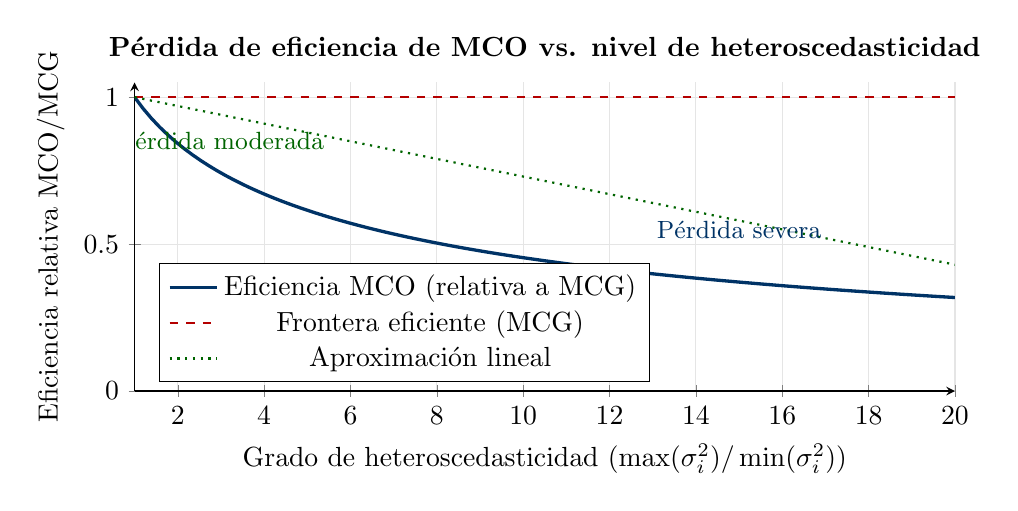
\begin{tikzpicture}
    \begin{axis}[
      width=12cm, height=5.5cm,
      xlabel={Grado de heteroscedasticidad ($\max(\sigma_i^2)/\min(\sigma_i^2)$)},
      ylabel={Eficiencia relativa MCO/MCG},
      title={\textbf{Pérdida de eficiencia de MCO vs. nivel de heteroscedasticidad}},
      xmin=1, xmax=20, ymin=0, ymax=1.05,
      grid=major, grid style={gray!20},
      axis lines=left,
      legend pos=south west,
    ]
      \addplot[azuloscuro, very thick, domain=1:20, samples=100] {1/(0.3*x^0.7+0.7)};
      \addlegendentry{Eficiencia MCO (relativa a MCG)}
      \addplot[rojoalerta, thick, dashed, domain=1:20] {1};
      \addlegendentry{Frontera eficiente (MCG)}
      \addplot[verdematematica, thick, dotted, domain=1:20, samples=100] {1 - 0.03*(x-1)};
      \addlegendentry{Aproximación lineal}
      \node[font=\small, azuloscuro] at (axis cs:15,0.55) {Pérdida severa};
      \node[font=\small, verdematematica] at (axis cs:3,0.85) {Pérdida moderada};
    \end{axis}
  \end{tikzpicture}
  \caption{A medida que el grado de heteroscedasticidad (razón entre la varianza máxima y mínima) aumenta, la eficiencia relativa de MCO respecto a MCG disminuye. Con homocedasticidad perfecta (ratio $= 1$), ambos estimadores son igualmente eficientes.}
  \label{fig:eficiencia}
\end{figure}

\chapter*{Resumen Ejecutivo del Capítulo 11}
\addcontentsline{toc}{chapter}{Resumen Ejecutivo}

\begin{tcolorbox}[enhanced, breakable, colback=azuloscuro!5, colframe=azuloscuro,
                  title={\Large\bfseries Síntesis: Heteroscedasticidad},
                  fonttitle=\color{white}]

  \textbf{\large 1. ¿Qué es?}

  La heteroscedasticidad ocurre cuando $\E(u_i^2) = \sigma_i^2 \neq \sigma^2$ (varianza no constante). Es típica en datos de corte transversal con unidades de tamaño muy diferente.

  \vspace{0.5cm}
  \textbf{\large 2. ¿Qué le pasa a MCO?}

  \begin{center}
  \begin{tabular}{lc}
    \toprule
    Propiedad & Estado \\
    \midrule
    Insesgadez & \textcolor{verdematematica}{\checkmark Conservada} \\
    Consistencia & \textcolor{verdematematica}{\checkmark Conservada} \\
    Eficiencia (BLUE) & \textcolor{rojoalerta}{\textbf{$\times$ Perdida}} \\
    Varianzas correctas & \textcolor{rojoalerta}{\textbf{$\times$ Incorrectas}} \\
    Pruebas $t$ y $F$ & \textcolor{rojoalerta}{\textbf{$\times$ Inválidas}} \\
    \bottomrule
  \end{tabular}
  \end{center}

  \vspace{0.5cm}
  \textbf{\large 3. ¿Cómo se detecta?}

  Gráficos de residuales $+$ Pruebas formales: Park, Glejser, Spearman, Goldfeld-Quandt, BPG, White.

  \vspace{0.5cm}
  \textbf{\large 4. ¿Cómo se corrige?}

  \begin{itemize}
    \item Si $\sigma_i^2$ conocida $\rightarrow$ \textbf{MCP} (óptimo, BLUE).
    \item Si $\sigma_i^2$ desconocida y muestra grande $\rightarrow$ \textbf{Errores robustos de White}.
    \item Si patrón identificable $\rightarrow$ \textbf{Transformaciones} (log, raíz cuadrada, razones).
  \end{itemize}

  \vspace{0.5cm}
  \textbf{\large 5. Fórmulas Clave}

  \begin{align*}
    \betahat_{GLS} &= (\mathbf{X}'\boldsymbol{\Omega}^{-1}\mathbf{X})^{-1}\mathbf{X}'\boldsymbol{\Omega}^{-1}\mathbf{y} &\text{(MCG)}\\
    \Var(\betahat_2)_{\text{verdadera}} &= \frac{\sum x_i^2\sigma_i^2}{(\sum x_i^2)^2} &\text{(Varianza real MCO)}\\
    W &= nR^2_{\text{aux}} \sim \chi^2_{(p)} &\text{(Prueba de White)}\\
    F_{GQ} &= \frac{RSS_2/(n_2-k)}{RSS_1/(n_1-k)} \sim F_{n_2-k,n_1-k} &\text{(Goldfeld-Quandt)}
  \end{align*}
\end{tcolorbox}

\end{document}
